\documentclass[conference]{IEEEtran}
% IEEE Conference Template downloaded from the user's Overleaf project.
\usepackage[T1]{fontenc}
\usepackage{cite}
\usepackage{amsmath,amssymb,amsfonts}
\usepackage{graphicx}
\usepackage{textcomp}
\usepackage{xcolor}
\usepackage[hidelinks]{hyperref}
\interdisplaylinepenalty=2500
\begin{document}
\title{Energy-Based Multi-Plane Segmentation of 3D Point Clouds}
\author{\IEEEauthorblockN{Matt (Haocun) Jing}
\IEEEauthorblockA{Department of Electrical and Computer Engineering\\
University of Victoria\\
ECE 503: Optimization in Machine Learning}}
\maketitle
\begin{abstract}
Plane segmentation requires estimating geometric models and their supporting points under measurement noise. This paper compares sequential random sample consensus (RANSAC), the energy-based multi-model fitting method PEARL with sampled proposals, and a hybrid that initializes PEARL with RANSAC planes and assignments. PEARL alternates graph-cut assignment updates with singular value decomposition for plane refitting, minimizing geometric error and spatial disagreement. Hyperparameters are selected on the training split of the Synthetic Plane Extraction Benchmark and fixed for evaluation on 30 test scans, four measurement variants, and three random seeds. Sampled PEARL achieves the highest mean matched point accuracy of 84.26\%, requiring 19.620 s per record. The hybrid achieves 77.98\% in 2.512 s, improving RANSAC accuracy by 8.08 percentage points while running approximately 7.81 times faster than sampled PEARL. RANSAC remains fastest at 0.376 s, with 69.89\% accuracy. Hybrid mean matched intersection over union is 0.2836, compared with 0.4554 for sampled PEARL, indicating a remaining difference in individual-plane recovery. A fixed-configuration ablation reduces sampled PEARL accuracy to 11.27\% when spatial regularization is removed. These results favor spatially regularized, RANSAC-initialized PEARL as a practical cost--accuracy compromise among the tested pipelines, while showing that lower fitting energy does not guarantee improved reference-label accuracy.
\end{abstract}
\begin{IEEEkeywords}
Energy minimization, graph cuts, plane segmentation, point clouds, random sample consensus.
\end{IEEEkeywords}
\section{Introduction}\label{introduction}

Extracting planar surfaces from three-dimensional point clouds is a fundamental task in computer vision and robotics. Walls, floors, and other approximately planar structures provide a compact description of an environment and geometric constraints for reconstruction, registration, and robot localization. Plane representations are particularly attractive in structured indoor scenes, where large surfaces can replace many individual point measurements in a map \cite{kaess2015planes,schaefer2019planes}. Reliable extraction therefore requires more than an accurate plane equation: the method must also identify the observations that support each surface while rejecting measurements that do not belong to any recovered plane.\footnote{The MATLAB source code, confirmed settings, and reproduction instructions for this comparison are publicly available on GitHub~\cite{jing2026planes}: \url{https://github.com/Mattjing/plane-segmentation}.}

This association is difficult because the supporting points are not known in advance. Measurement noise perturbs surface geometry, occlusion produces incomplete observations, and clutter introduces competing structures and outliers. Near the intersection of two planes, a point may be consistent with more than one model. Unequal surface sizes further complicate estimation because a small plane can be obscured by the support of a larger neighboring surface. Although three non-collinear points determine a plane, a noisy or mixed sample may produce an unreliable hypothesis. Conversely, fitting a model to all observations can combine several distinct surfaces. The problem is a joint optimization over continuous plane parameters and discrete point-to-plane assignments. Unlike a classifier that learns reusable weights, it estimates the models and their supporting point sets anew for each scan.

Random Sample Consensus (RANSAC), introduced by Fischler and Bolles \cite{fischler1981ransac}, addresses robust model estimation by drawing small subsets of observations and evaluating the support of the resulting hypotheses. For plane extraction, three non-collinear sampled points generate a candidate plane. The candidate is tested against all available points using orthogonal point-to-plane distances, and its consensus set contains those within a specified tolerance. Repeated sampling increases the opportunity to obtain a hypothesis from points on the same surface. The candidate with the largest support can then be refined by least-squares fitting to its inliers. This procedure is simple to implement and can tolerate substantial outlier contamination when a sufficiently supported model is present.

Sequential RANSAC extends this procedure to multiple planes by extracting one model, removing its inliers, and repeating the search on the remaining observations. Its direct computation and explicit geometric threshold make it a useful baseline. However, the extraction is greedy: points assigned to an early plane are unavailable to later models, and an erroneous removal can distort the remaining segmentation. Small surfaces may be missed when their support is weak, while threshold choices can cause neighboring surfaces to merge or individual surfaces to fragment. The sampling effort also increases as useful consensus sets become harder to find. These limitations motivate methods that reconsider assignments across several candidate models.

A later alternative is the PEARL framework of Isack and Boykov, published in 2012 \cite{isack2012energy}. PEARL begins with sampled model hypotheses but formulates their estimation as the minimization of a common energy. Its basic formulation combines geometric fitting costs with a spatial regularity term that discourages inconsistent labels among neighboring observations. For fixed models, \(\alpha\)-expansion updates the assignments through graph-cut moves \cite{boykov2001graphcuts}. For fixed assignments, the model parameters are re-estimated from their supporting points. Repeating these steps allows observations to move between competing models and improves the models beyond their original sampled estimates. For the squared orthogonal plane-fitting costs used here, re-estimation is performed by least-squares fitting using singular value decomposition.

The flexibility of joint reassignment introduces additional computational work. In our implementation, each \(\alpha\)-expansion sweep attempts a move for every candidate label, and each move requires constructing and solving a binary cut problem over the point neighborhood graph. These sweeps are repeated as the plane parameters change, alongside the evaluation of fitting costs and the least-squares updates. Runtime consequently depends on the number of points, graph edges, candidate planes, and optimization iterations. The solution also depends on initialization and regularization strength, and global optimality is not guaranteed \cite{isack2012energy}. Spatial coherence can resolve ambiguous assignments, but excessive regularization can suppress valid boundaries. Energy reduction alone therefore does not establish agreement with a reference segmentation.

This paper examines these accuracy and computational tradeoffs through a MATLAB implementation on the Synthetic Plane Extraction Benchmark (SynPEB) \cite{schaefer2019planes}. The study compares sequential RANSAC, PEARL initialized with sampled proposals, and a hybrid that applies PEARL refinement to the planes and assignments produced by RANSAC. It also removes spatial regularization to assess its role under otherwise fixed settings. Hyperparameters are selected using training scans and then held fixed during independent fitting of each test scan; no plane classifier is learned across scans. Evaluation uses reference plane memberships, matched segmentation metrics, repeated random seeds, energy histories, and algorithm runtimes. The aim is to determine when joint optimization improves greedy extraction and how much of the outcome depends on the initial model set.

\section{Related Work}\label{related-work}

Methods for fitting multiple geometric structures differ primarily in how they couple model estimation with point grouping. Consensus methods search for hypotheses supported by many observations, preference-based methods group points according to their agreement with sampled models, and energy-based methods optimize an explicit objective over assignments and model parameters. These alternatives provide the context for comparing sequential RANSAC with PEARL.

RANSAC \cite{fischler1981ransac} established the hypothesis-and-verification approach to robust estimation, in which a model generated from a minimal sample is assessed by its consensus set. Subsequent work has examined how refinement can improve the reliability of sampled estimates. Chum, Matas, and Kittler \cite{chum2003locally} observed that even an outlier-free sample need not produce a model consistent with all true inliers under measurement noise. Their locally optimized RANSAC (LO-RANSAC) refines promising hypotheses to improve support. This demonstrates the importance of distinguishing a sampled hypothesis from its refined estimate. However, improving one model does not itself resolve the competition among several structures. Sequential extraction still commits points to earlier models before later surfaces are considered. The least-squares refinement used in our baseline follows this general motivation but is not an implementation of the complete LO-RANSAC algorithm.

Preference-based clustering addresses multiple structures by representing how each observation agrees with a collection of hypotheses. Toldo and Fusiello \cite{toldo2008jlinkage} introduced J-linkage, which describes a point by the set of sampled models consistent with it and groups points using agglomerative clustering in this preference space. Magri and Fusiello \cite{magri2014tlinkage} extended this idea through T-linkage, replacing binary preferences with a continuous representation. Their distinction is relevant near uncertain inlier boundaries, where a hard threshold discards differences in residual magnitude. These methods group observations through shared model preferences rather than repeatedly removing the strongest consensus set. Their central representation is nevertheless different from the explicit spatially regularized assignment energy studied here.

Energy-based fitting makes the relationship between data association and model estimation explicit. Isack and Boykov \cite{isack2012energy} formulate multi-model fitting through geometric error and regularization, and introduce PEARL to alternate assignment optimization with model re-estimation. For a fixed candidate set, the assignment stage uses the \(\alpha\)-expansion framework of Boykov, Veksler, and Zabih \cite{boykov2001graphcuts}, allowing many observations to change labels within a move. The continuous fitting stage then updates the geometric parameters using the current groups. This combination is important because neither a fixed proposal pool nor a single pass of point assignment fully addresses their mutual dependence. PEARL provides an iterative strategy for reducing the same objective across both updates, while retaining dependence on initialization and local solutions.

The choice of regularization determines which properties an energy favors. Spatial smoothness penalizes neighboring observations that receive different labels, whereas a label cost penalizes the use of models themselves. Delong et al. \cite{delong2012labelcosts} developed an extension of \(\alpha\)-expansion that accommodates such label costs, providing a mechanism for discouraging unnecessary model complexity. These terms should not be conflated: coherent point groups do not imply that the number of models is explicitly penalized. Our implementation adopts the basic geometric-error and neighborhood formulation of PEARL, without an additional model-count term. Consequently, its plane-count cap is a computational setting rather than an optimized complexity penalty.

The computational cost of discrete assignment optimization has also motivated continuous alternatives. Amayo et al. \cite{amayo2018coral} proposed CORAL, which relaxes discrete point memberships into soft assignments and optimizes a global fitting energy using a formulation suitable for parallel computation. Their evaluation includes plane extraction from RGB-D data and homography estimation. This work shows that the energy formulation and the numerical solver are distinct design choices: similar geometric objectives can be approached through different assignment representations. It also motivates examining runtime alongside segmentation quality. The present study retains graph-cut-based expansion, while CORAL illustrates an alternative approach to assignment optimization.

Plane extraction is also shaped by the sensor model and the intended application. Kaess \cite{kaess2015planes} demonstrates the use of plane landmarks in simultaneous localization and mapping, while Schaefer et al. \cite{schaefer2019planes} estimate finite planes through a probabilistic treatment of laser measurements that incorporates ray information. The latter work also introduces SynPEB for quantitative evaluation. Our experiments use the supplied point coordinates and reference plane memberships, without adopting that measurement-likelihood formulation. Within this scope, we compare greedy extraction, sampled-proposal PEARL, and RANSAC-initialized PEARL to examine the effects of joint reassignment, initialization, and spatial regularization. J-linkage, T-linkage, LO-RANSAC, label-cost extensions, and CORAL provide methodological context rather than additional experimental baselines.

\section{RANSAC and Sequential RANSAC}\label{ransac-and-sequential-ransac}

Sequential RANSAC extracts a collection of planes by repeatedly applying a single-model consensus search to the points that remain unassigned. This section specifies the implemented pipeline: generate a plane from a sampled triplet, measure its support over all remaining points, refine the strongest candidate, and remove its accepted support before searching for another plane. The single-model search follows the robust estimation principle of RANSAC \cite{fischler1981ransac}.

\subsection{Plane representation and estimation task}\label{plane-representation-and-estimation-task}

Let P = \{\(x_{1}\), \ldots, \(x_{n}\)\} be the input point cloud, with each observation in three-dimensional Euclidean space. A plane is represented by a normal n and signed offset d:

\begin{equation}
n^\top x+d=0,\qquad \|n\|_2=1.
\label{eq:1}
\end{equation}

The unit-normal constraint makes the absolute algebraic residual equal to the orthogonal point-to-plane distance. For plane \(\theta\) = (n, d), define

\begin{equation}
r_i(\theta)=|n^\top x_i+d|.
\label{eq:2}
\end{equation}

The unknowns are the plane parameters and the membership of each point. They are estimated separately for every scan; no classifier weights are trained or transferred between scans. Reference plane IDs are used only for parameter selection and evaluation, never to construct a hypothesis or select its inliers. The output labels are temporary identifiers assigned in extraction order, rather than semantic classes learned from reference IDs.

\subsection{Hypothesis generation from three points}\label{hypothesis-generation-from-three-points}

At extraction stage k, let \(R_{k}\) denote the indices of the remaining points. Each trial draws three distinct indices from this set. In the implementation, sampling is local with probability \(\rho\) and global with probability 1 \(-\) \(\rho\). A local draw first selects a remaining anchor, then draws a triplet from remaining points inside a square patch of radius h in the organized, subsampled scan grid. If fewer than three points are available in that patch, the draw falls back to global sampling. Global sampling draws a triplet uniformly without replacement from \(R_{k}\). Locality uses grid position and does not require reference labels.

For sampled coordinates a, b, and c, the geometric construction is

\begin{equation}
v=(b-a)\times(c-a),
\label{eq:3}
\end{equation}

\begin{equation}
n=\frac{v}{\|v\|_2},\qquad d=-n^\top a.
\label{eq:4}
\end{equation}

A collinear triplet does not determine a unique plane and must be rejected. The code computes the equivalent plane through a centered singular value decomposition (SVD), rather than explicitly using the cross product. It rejects a sample if the second singular value is below \(1^{-10}\), which detects coincident or numerically collinear samples. It also fixes the normal sign so that its component with greatest absolute magnitude is positive. Changing both n and d to their negatives would represent the same plane.

\subsection{Consensus scoring and the inner loop}\label{consensus-scoring-and-the-inner-loop}

A triplet generates a hypothesis; it does not supply the complete inlier set. Every valid candidate is verified against every remaining point. Given the fixed distance threshold \(\tau\), the consensus set is

\begin{equation}
I_k(\theta)=\{i\in R_k:r_i(\theta)\leq\tau\}.
\label{eq:5}
\end{equation}

The support count and residual score are

\begin{equation}
S_k(\theta)=|I_k(\theta)|,
\label{eq:6}
\end{equation}

\begin{equation}
Q_k(\theta)=\sum_{i\in I_k(\theta)}r_i^2(\theta).
\label{eq:7}
\end{equation}

The inner loop retains the candidate with greatest support. If two candidates have equal support, the one with the smaller sum of squared inlier distances is retained. This is a lexicographic selection rule: support count has priority over fitting error. It is neither softmax classification nor an independent nearest-plane assignment. Sampling approximates a maximum-consensus search; it does not guarantee the globally best plane.

The current implementation performs T = 150 attempted hypotheses per extracted plane. Degenerate attempts consume a trial and are skipped without scoring. Once all attempts have been processed, extraction terminates if the strongest candidate has fewer than m supporting points. Otherwise, its parameters and support initialize the refinement stage. T is a fixed computational budget, and the code does not adapt it using a desired success probability.

\subsection{Refinement using the consensus set}\label{refinement-using-the-consensus-set}

Three points suffice to propose a plane, but measurement noise makes such an estimate sensitive to the sampled locations. Refinement uses all currently accepted inliers to solve the constrained orthogonal least-squares problem

\begin{equation}
\min_{\|n\|_2=1,\,d}\;\sum_{i\in I}(n^\top x_i+d)^2.
\label{eq:8}
\end{equation}

Let \(\mu\) be the centroid of these inliers and A the matrix whose rows are their centered coordinates:

\begin{equation}
\mu=\frac{1}{|I|}\sum_{i\in I}x_i,\qquad A_{i,:}=(x_i-\mu)^\top.
\label{eq:9}
\end{equation}

For the decomposition A = U\(\Sigma\)\(V^{T}\), the right singular vector associated with the smallest singular value minimizes the orthogonal least-squares objective:

\begin{equation}
n=v_{\min},\qquad d=-n^\top\mu.
\label{eq:10}
\end{equation}

After each refit, distances are recomputed for all points in \(R_{k}\), including those outside the previous consensus set. Points can therefore enter or leave the candidate support. Up to three refit-and-reclassification passes are performed. If a refit is degenerate or its new support falls below m, the pass is rejected and the last accepted plane and support are retained. The code does not stop early merely because membership is unchanged.

For fixed membership, SVD minimizes the squared fitting error. Reclassification changes that membership, however, so the complete refinement loop is not guaranteed to monotonically improve the earlier lexicographic score. The stored plane is fitted to the support entering the last accepted pass; its returned support is obtained by thresholding that plane. This describes the implemented ordering without assuming an additional final refit.

\subsection{Sequential extraction and stopping rules}\label{sequential-extraction-and-stopping-rules}

Initialize \(R_{1}\) to all input indices and assign every point label zero. After the inner search and refinement accept a plane \(\theta_{k}\) with support \(I_{k}\), update the labels and remaining set as follows:

\begin{equation}
L_i=k\quad\text{for }i\in I_k,
\label{eq:11}
\end{equation}

\begin{equation}
R_{k+1}=R_k\setminus I_k.
\label{eq:12}
\end{equation}

The next outer iteration runs a fresh hypothesis search on this reduced set. Previously accepted planes and their assigned points are not revisited. The procedure stops when fewer than m points remain, the best new candidate has fewer than m inliers, or the number of extracted planes reaches the cap \(K_{max}\). Unassigned points retain label zero. The cap is a computational limit and does not use the reference number of planes.

The loop structure is therefore: initialize the remaining set; perform T hypothesis attempts; retain the strongest candidate; reject insufficient support or refine it up to three times; assign and remove its inliers; and repeat until an outer stopping rule is met. With \(N_{k}\) remaining points at stage k, candidate verification requires O(T\(N_{k}\)) residual evaluations. The total verification work scales as \(O(T\sum_k N_k)\), in addition to sampling and SVD refinement.

\subsection{Fixed settings and practical limitations}\label{fixed-settings-and-practical-limitations}

RANSAC requires no supervised fitting phase, but it does require algorithm settings: \(\tau\), T, m, \(K_{max}\), \(\rho\), and h. In this project, the training split was used to select shared settings, including the distance threshold, minimum support, plane cap, and local radius, before test evaluation. The hypothesis budget and local sampling fraction were fixed. All selected settings remain unchanged during testing, while plane parameters and memberships are estimated anew for each scan. Thus, absence of learned weights does not imply absence of hyperparameter selection.

The threshold controls the tradeoff between tolerance to noise and incorrect support from nearby surfaces. A larger trial budget increases the opportunity to sample a useful plane but increases runtime. Greedy removal makes sequential RANSAC efficient and simple, while preventing later evidence from correcting an earlier assignment. Points near intersections may support more than one plane, and early extraction can deprive a smaller surface of sufficient support. These limitations motivate the joint reassignment and model re-estimation considered in the following PEARL section.

\section{PEARL for Joint Plane Estimation and Segmentation}\label{pearl-for-joint-plane-estimation-and-segmentation}

PEARL couples geometric model estimation with the assignment of observations to models. Isack and Boykov \cite{isack2012energy} proposed an energy-based framework in which sampled hypotheses initialize a finite model set, assignment optimization estimates their spatial support, and refitting updates their parameters. Our implementation adapts this alternating strategy to three-dimensional plane segmentation. It uses squared orthogonal distances and a weighted Potts spatial prior, with an explicit outlier label. The model-count penalty discussed in the PEARL literature and label-cost extensions \cite{delong2012labelcosts} is not included.

The goal is to minimize a single energy that balances geometric fit against the cost of assigning different labels to neighboring points. Starting from the initial planes and labels, the algorithm alternates between \(\alpha\)-expansion, which updates the labels while holding the planes fixed, and singular value decomposition (SVD), which refits the planes while holding the labels fixed. After each full iteration, the algorithm checks how much the normalized energy has decreased. If the decrease is no greater than the tolerance \(\varepsilon\), it stops early. This stopping rule does not guarantee that the global minimum has been reached.

\subsection{Unknowns and the energy function}\label{unknowns-and-the-energy-function}

For N input points, let \(\Theta\) = \{\(\theta_{1}\), \ldots, \(\theta_{m}\)\} be the current plane bank. Each \(\theta_{k}\) = (\(n_{k}\), \(d_{k}\)) has a unit normal, as in Section~\ref{ransac-and-sequential-ransac}. The assignment vector L contains one label per point: \(L_{i}\) \(\in\) \{0, 1, \ldots, M\}. Label k \textgreater{} 0 selects plane \(\theta_{k}\); label zero designates an outlier. The joint estimation problem is

\begin{equation}
\min_{L,\Theta}\;E(L,\Theta),\qquad \forall k:\|n_k\|_2=1.
\label{eq:13}
\end{equation}

The implemented objective has two terms:

\begin{equation}
\begin{aligned}E(L,\Theta)&=\sum_{i=1}^{N}D_i(L_i;\Theta)\\&\quad+\lambda\sum_{(i,j)\in\mathcal E}w_{ij}[L_i\ne L_j].\end{aligned}
\label{eq:14}
\end{equation}

Here \(\mathcal E\) is a fixed neighborhood edge set, \(w_{ij}\) \(\geq\) 0 is an edge weight, and the bracket is an indicator equal to one when its condition holds. The unary data costs are

\begin{equation}
D_i(k;\Theta)=(n_k^\top x_i+d_k)^2,\quad k>0,
\label{eq:15}
\end{equation}

\begin{equation}
D_i(0;\Theta)=\tau^2,\qquad\lambda=\eta\tau^2.
\label{eq:16}
\end{equation}

The first term measures how well each point fits its assigned plane. For a point assigned to a plane, the cost is the squared perpendicular distance to that plane, with no cap. A point labeled as an outlier instead incurs a fixed cost of \(\tau^{2}\). The second term compares the labels of points joined by an edge in the neighborhood graph. An edge adds no cost if its endpoints have the same label and adds a weighted penalty if their labels differ, whether they belong to two different planes or one is an outlier. For example, at a wall--floor corner, the optimizer can assign connected points to different planes if the reduction in squared-distance costs outweighs the added boundary penalty.

For numerical stability, our work divides the entire objective by \(\tau^{2}\), giving

\begin{equation}
\begin{aligned}\bar E(L,\Theta)&=\frac{E(L,\Theta)}{\tau^2}=\sum_i\frac{D_i(L_i;\Theta)}{\tau^2}\\&\quad+\eta\sum_{(i,j)\in\mathcal E}w_{ij}[L_i\ne L_j].\end{aligned}
\label{eq:17}
\end{equation}

Since \(\tau\) \textgreater{} 0, this positive scaling preserves every minimizer. The normalized outlier cost is one and \(\eta\) is the smoothness ratio stored as \texttt{lambdaRatio}. The reported energy histories multiply normalized values by \(\tau^{2}\) to recover the original units. No softmax or learned classifier is involved.

\subsection{The neighborhood graph}\label{the-neighborhood-graph}

The graph is constructed once from the organized scan after subsampling. Candidate edges join horizontally or vertically adjacent valid grid positions. An edge is discarded if the Euclidean separation between its points exceeds \(r_{max}\). For retained edges,

\begin{equation}
w_{ij}=\exp\!\left(-\frac{\|x_i-x_j\|_2^2}{2\sigma^2}\right).
\label{eq:18}
\end{equation}

The spatial scale \(\sigma\) controls how quickly coupling decays with three-dimensional separation, while \(r_{max}\) removes long edges across depth jumps. The selected configuration uses \(\sigma\) = 0.15 and \(r_{max}\) = 0.30 in the supplied coordinate units. Sampling stride eight retains every eighth row and column; it affects point count, graph connectivity, and the physical separation between neighbors. Reference annotations do not enter edge construction. Neither adjacency nor a shared surface guarantees equal reference IDs: the graph expresses a prior, not a rule defining the dataset labels.

\subsection{Hypotheses and initial assignments}\label{hypotheses-and-initial-assignments}

The sampled-proposal variant attempts H = 1,000 plane hypotheses before optimization. Each attempt uses the same mixed sampler as sequential RANSAC: local sampling with probability \(\rho\) = 0.7, otherwise global sampling. A local draw uses a square grid patch of radius h = 8 and falls back to a global draw if the patch contains fewer than three available points. All input points remain available throughout proposal generation. Triplet parameters can be written as

\begin{equation}
v=(b-a)\times(c-a),
\label{eq:19}
\end{equation}

\begin{equation}
n=\frac{v}{\|v\|_2},\qquad d=-n^\top a.
\label{eq:20}
\end{equation}

The implementation obtains the equivalent parameters through centered SVD and rejects triplets with second singular value below \(1^{-10}\). A valid proposal is retained only if at least m = 6 input points lie within \(\tau\) = 0.04 of it. Candidates are ranked by this thresholded support. Redundant candidates are suppressed using angular and sign-aligned offset differences:

\begin{equation}
\varphi_{ab}=\arccos(|n_a^\top n_b|),
\label{eq:21}
\end{equation}

\begin{equation}
\Delta_{ab}=|d_a-\operatorname{sign}(n_a^\top n_b)d_b|.
\label{eq:22}
\end{equation}

A candidate is skipped if any already retained plane has angle below 3\({}^\circ\) and offset difference below 0.015. Up to M = 150 distinct candidates are retained. This suppression occurs before optimization and does not merge final segments. Initial labels minimize the unary costs independently:

\begin{equation}
L_i^{(0)}\in\operatorname*{arg\,min}_{k\in\{0,\ldots,M\}}D_i(k;\Theta^{(0)}).
\label{eq:23}
\end{equation}

This initialization ignores pairwise costs. Subsequent expansion moves introduce spatial coupling. The hybrid method initializes PEARL with the planes and point labels returned by sequential RANSAC, then applies the same energy and optimization updates as the sampled-proposal variant. Its design is described in Section~\ref{hybrid-ransac-and-pearl-method}.

\subsection{Assignment optimization by alpha expansion}\label{assignment-optimization-by-alpha-expansion}

With \(\Theta\) fixed, \(\alpha\)-expansion \cite{boykov2001graphcuts} considers one target label \(\alpha\) at a time. A binary variable \(z_{i}\) determines whether point i keeps its current label or switches to \(\alpha\):

\begin{equation}
L_i(z_i)=(1-z_i)L_i+z_i\alpha,
\label{eq:24}
\end{equation}

\begin{equation}
z_i\in\{0,1\},\qquad\alpha\in\{0,\ldots,M\}.
\label{eq:25}
\end{equation}

Label arithmetic in this expression encodes the two choices only; numerical label values have no geometric ordering. A single move solves

\begin{equation}
z^*\in\operatorname*{arg\,min}_{z\in\{0,1\}^N}\bar E(L(z),\Theta).
\label{eq:26}
\end{equation}

Thus, an expansion may change any subset of points to one candidate plane while the other points retain their current labels. It does not update plane parameters. Many points can switch together, including disconnected groups if that lowers energy. The binary problem is solved exactly by a minimum cut, but the complete multi-label and continuous problem is only approximately optimized. A move is accepted only if it lowers the normalized energy by more than \(\varepsilon\) = \(1^{-9}\).

The graph-cut construction can be made explicit for this implementation. Let \(v_{ij}\) = \(\eta\)\(w_{ij}\) and let A, B, and C denote the current labels of points i and j and the target \(\alpha\), respectively. The four pairwise costs for binary states are

\begin{equation}
e_{00}=v_{ij}[A\ne B],\qquad e_{11}=0,
\label{eq:27}
\end{equation}

\begin{equation}
e_{01}=v_{ij}[A\ne C],\qquad e_{10}=v_{ij}[C\ne B].
\label{eq:28}
\end{equation}

The Potts disagreement indicator satisfies the triangle inequality, so these costs obey the binary submodularity condition required for graph representation \cite{kolmogorov2004energy}:

\begin{equation}
e_{00}+e_{11}\leq e_{01}+e_{10}.
\label{eq:29}
\end{equation}

The code decomposes each edge cost into a constant, two unary corrections, and a nonnegative cut term:

\begin{equation}
V(z_i,z_j)=e_{00}+az_i+bz_j+c|z_i-z_j|,
\label{eq:30}
\end{equation}

\begin{equation}
c=\frac{e_{01}+e_{10}-e_{00}}{2}\geq0,
\label{eq:31}
\end{equation}

\begin{equation}
a=e_{10}-e_{00}-c,\qquad b=e_{01}-e_{00}-c.
\label{eq:32}
\end{equation}

Unary corrections are accumulated at their endpoints. At each point, subtracting the smaller of the two resulting unary costs preserves the optimizer and makes terminal capacities nonnegative. The graph then has one node per point, source and sink terminals for keep and switch, and edges of capacity c between neighbors. MATLAB \texttt{maxflow} obtains the minimum cut. This gives an exact solution for the current binary move, rather than an exhaustive search over all multi-label assignments.

\subsection{Model re-estimation by SVD}\label{model-re-estimation-by-svd}

After expansion, memberships are fixed and each plane is refitted to its assigned support \(I_{k}\) = \{i : \(L_{i}\) = k\}. For each valid support containing at least three points, the continuous subproblem is

\begin{equation}
\min_{\|n_k\|_2=1,\,d_k}\;\sum_{i\in I_k}(n_k^\top x_i+d_k)^2.
\label{eq:33}
\end{equation}

Let \(\mu_{k}\) be the support centroid and \(A_{k}\) the matrix of centered point coordinates. Differentiation with respect to \(d_{k}\) gives the optimal offset, reducing the problem to a constrained quadratic form:

\begin{equation}
d_k=-n_k^\top\mu_k,
\label{eq:34}
\end{equation}

\begin{equation}
\begin{aligned}\min_{\|n_k\|_2=1}\|A_kn_k\|_2^2&=\min_{\|n_k\|_2=1}n_k^\top A_k^\top A_kn_k.\end{aligned}
\label{eq:35}
\end{equation}

For \(A_{k}\) = \(U_{k}\)\(\Sigma_{k}\)\(V_{k}^{T}\), the solution is the right singular vector associated with the smallest singular value. Equivalently, it is the unit eigenvector of \(A_{k}^{T}\)\(A_{k}\) with smallest eigenvalue:

\begin{equation}
n_k=v_{k,\min},\qquad d_k=-n_k^\top\mu_k.
\label{eq:36}
\end{equation}

SVD reduces the first, geometric term of the energy. It does not reduce the second, spatial term directly: with L fixed, all disagreement indicators and edge weights remain unchanged. The outlier contribution is also constant. A nondegenerate refit can therefore lower the joint energy without changing any label. The code accepts it only if its normalized fitting cost does not exceed the previous cost by more than \(1^{-12}\). Supports with fewer than three points, or with a degenerate SVD, keep their previous plane parameters. Minimum proposal support m is not imposed again as a final segment-size filter.

\subsection{Why the two updates are coupled}\label{why-the-two-updates-are-coupled}

Assignments determine which observations enter each SVD. Updated parameters then change the data costs used by the next expansion. For exact non-increasing updates, this alternating relationship gives

\begin{equation}
\begin{aligned}E(L^{t+1},\Theta^{t+1})&\leq E(L^{t+1},\Theta^t)\\&\leq E(L^t,\Theta^t).\end{aligned}
\label{eq:37}
\end{equation}

The implementation enforces this behavior up to numerical tolerances. A coherent group can first obtain a better assignment, then provide a more stable plane estimate than its original triplet, allowing further points to join in a later iteration. Conversely, an incorrect group can bias a refit and trap subsequent assignments. Decreasing energy improves the specified compromise between fit and coherence; it does not guarantee that both terms decrease independently, nor that ground-truth accuracy increases. The reference labels are absent from this objective.

\subsection{The complete loop and iteration limits}\label{the-complete-loop-and-iteration-limits}

The pipeline follows the four PEARL operations, with the following implementation-specific limits.

\begin{enumerate}
\item \textbf{Propose.} Generate and screen the initial candidate bank once, or accept the exact sequential-RANSAC planes and labels. For sampled initialization, compute unary-minimum labels. Evaluate the complete initial energy before any expansion.

\item \textbf{Expand.} Keep all plane parameters fixed. Perform up to three sweeps; in each sweep, visit every plane label and the outlier label once, in a newly randomized order. For each target, solve one binary cut and accept a sufficiently energy-reducing move. End the sweep loop early if a complete sweep fails to improve normalized energy by more than \(\varepsilon\).

\item \textbf{Re-estimate.} Keep the resulting labels fixed and attempt one SVD refit for every plane. Recompute the full unary matrix and complete energy after the refits. No new candidate planes are proposed, and unused candidates remain available during optimization.

\item \textbf{Repeat.} Alternate expansion and refitting for at most 15 outer iterations. Stop early if the normalized energy reduction across a complete outer iteration is at most \(\varepsilon\). After stopping, remove only unused labels and compact their IDs. No final reassignment, segment merging, or support filtering is applied.

\end{enumerate}

Three sweeps means three passes over all labels, not three individual \(\alpha\)-expansion moves. With M plane labels, the maximum number of binary moves is

\begin{equation}
N_{\mathrm{cuts}}\leq15\times3\times(M+1).
\label{eq:38}
\end{equation}

For M = 150, this bound is 6,795 graph cuts; early stopping usually reduces it. The energy log contains the initial state and one entry after expansion and refitting for every completed outer iteration, giving at most 31 values. Reaching the iteration or sweep cap does not establish convergence to an expansion-local minimum. The random seed controls both proposal sampling and label-visit order.

\subsection{Hyperparameter effects and interactions}\label{hyperparameter-effects-and-interactions}

The energy parameters are \(\tau\), \(\eta\), \(\sigma\), and the graph cutoff \(r_{max}\). The threshold \(\tau\) sets the outlier penalty and is also used to screen proposals. Increasing it makes outlier assignment more costly, admits broader proposal support, and, at fixed \(\eta\), increases the physical smoothness weight \(\lambda\) = \(\eta\)\(\tau^{2}\). It therefore changes several parts of the pipeline together. The selected values \(\tau\) = 0.04 and \(\eta\) = 0.4 imply \(\lambda\) = 0.00064 and an outlier cost of 0.0016. Unlike proposal screening, final assignment does not enforce \(\tau\) as a hard distance bound: spatial savings can justify assigning a point whose plane residual exceeds \(\tau\).

The ratio \(\eta\) controls coherence relative to normalized fitting error. At \(\eta\) = 0, assignment for fixed planes separates into independent unary minima; alternating these assignments and SVD becomes a spatially unregularized fitting procedure. Increasing \(\eta\) discourages isolated assignments and fragmented support, but can also merge nearby structures or erase a small plane. The prior favors equal model labels, not merely similar normals. Distinct labels incur a boundary cost even if their planes are nearly parallel.

Increasing \(\sigma\) strengthens retained edges at a given separation. Increasing \(r_{max}\) adds candidate connections that would otherwise be removed, potentially coupling points across depth discontinuities. Neither change repairs a missing candidate plane. Proposal count H and candidate cap M control initialization coverage and optimization cost; local radius h and fraction \(\rho\) control the chance of sampling a coherent surface rather than crossing several surfaces. Angular and offset suppression tolerances determine how similar two candidates may be before one is discarded. These are initialization settings, rather than extra terms in the energy.

For a region R switching to \(\alpha\), let \(L^{'}\) denote the resulting labels and let \(\delta_{ij}\)(L) = {[}\(L_{i}\) \(\ne\) \(L_{j}\){]}. With \(\Theta\) fixed, the energy change explicitly balances fit and boundary changes:

\begin{equation}
\begin{aligned}\Delta E&=\sum_{i\in R}[D_i(\alpha)-D_i(L_i)]\\&\quad+\lambda\sum_{(i,j)\in\mathcal E}w_{ij}\bigl(\delta_{ij}(L')-\delta_{ij}(L)\bigr).\end{aligned}
\label{eq:39}
\end{equation}

Switching a coherent region may create only a boundary penalty while improving the fit of many interior points. Alternatively, a slight increase in fitting error can be accepted if removing label boundaries saves more spatial cost. If improved membership gives SVD cleaner support, the next geometric update may recover some of that fit cost. Strong smoothing applied to an incorrect initial group can instead reinforce the wrong model. More iterations cannot guarantee recovery from such a configuration.

The normalized stopping tolerance \(\varepsilon\) = \(1^{-9}\) controls acceptance and early stopping, not geometric accuracy. The iteration and sweep budgets limit optimization effort. All geometric scales use the input coordinate units; changing units requires corresponding changes to \(\tau\), \(\sigma\), \(r_{max}\), and the offset suppression tolerance. Scaling all lengths consistently and keeping \(\eta\) fixed scales the unnormalized energy by the square of the length conversion, while preserving the normalized objective.

\subsection{Hyperparameter selection on the training split}\label{hyperparameter-selection-on-the-training-split}

Hyperparameter selection is an outer experimental procedure, distinct from the per-scan energy minimization. It uses annotated training scans to choose settings, then fixes those settings before testing. There is no training of a reusable plane bank, assignment function, or network. Test scans generate and optimize their own hypotheses without reference labels.

Screening uses training scans 1 and 2, variants var1 and var4, and seed 7. A staged coordinate search first varies proposal count over \{1,000, 3,000, 5,000\}, plane cap over \{60, 100, 150\}, and local radius over \{2, 4, 8\}, carrying forward the selected configuration after each stage. It then evaluates the 25 threshold--smoothness combinations

\begin{equation}
\tau\in\{0.005,0.01,0.02,0.04,0.08\},
\label{eq:40}
\end{equation}

\begin{equation}
\eta\in\{0,0.02,0.05,0.15,0.4\},
\label{eq:41}
\end{equation}

and finally tests minimum proposal/extraction support m \(\in\) \{6, 12, 20\}. Previously completed configurations are reused. This staged search is not an exhaustive Cartesian search over every setting. The three highest-ranked screened configurations are confirmed on the disjoint training scans 3--10, using all four variants and seeds 7, 19, and 43: 96 scan--variant--seed records per configuration and method.

For a configuration c, the primary selection score gives the two methods equal weight:

\begin{equation}
J(c)=\tfrac12\bigl(\overline{\mathrm{IoU}}_{\mathrm{RANSAC}}^{\,c}+\overline{\mathrm{IoU}}_{\mathrm{PEARL}}^{\,c}\bigr).
\label{eq:42}
\end{equation}

Each method's mean is taken over the evaluated records. Per record, mean matched IoU averages reference-plane overlaps after one-to-one maximum-overlap matching, with unmatched reference planes contributing zero. Ties in J are resolved by greater mean F-score averaged across the two methods, then by smaller summed mean runtime. Raw energies are not compared across configurations with different parameters, and PEARL accuracy alone does not determine the winner.

Confirmation selected H = 1,000, M \(\leq\) 150, h = 8, m = 6, \(\tau\) = 0.04, and \(\eta\) = 0.4. The joint confirmation score was 0.3850. The alternative \(\tau\) = 0.08, \(\eta\) = 0.15 had greater PEARL-only matched IoU but a lower joint score. This distinction follows from selecting a shared experimental configuration. The remaining settings described above were fixed rather than searched. The spatial-prior ablation sets \(\eta\) to zero while retaining the sampled initialization; it tests the effect of removing spatial coupling under the selected configuration, rather than the best independently tuned unregularized model.

\subsection{Computation and limitations}\label{computation-and-limitations}

Proposal verification requires approximately O(HN) distance calculations. For a fixed bank of M planes, the unary matrix occupies O(N(M + 1)) memory. Each expansion builds and solves a binary graph with N point nodes and O(N + \textbar \(\mathcal E\)\textbar) arcs; its cost depends on the graph and max-flow solver. Repeating this operation across labels and sweeps is the principal extra work relative to greedy extraction. Refitting uses SVD of matrices with three columns, while refreshing the unary matrix again requires O(NM) residual evaluations.

Energy minimization supplies an explicit and auditable optimization target, but its success depends on the initial candidates, graph, noise scales, and computation budget. The implementation does not explicitly penalize the number of active planes. Unused labels disappear only at the end, and an active plane may have fewer than m assigned points. Neither low energy nor termination guarantees recovery of the reference segmentation, correct model count, or global optimality. These limits motivate measuring overlap, extracted-plane count, runtime, and energy reduction together.

\section{Hybrid RANSAC and PEARL Method}\label{hybrid-ransac-and-pearl-method}

The hybrid pipeline uses sequential RANSAC to construct an initial segmentation and PEARL to refine that complete solution. It combines the consensus search described in Section~\ref{ransac-and-sequential-ransac} with the joint assignment and model updates of Section~\ref{pearl-for-joint-plane-estimation-and-segmentation}, based on RANSAC \cite{fischler1981ransac}, PEARL \cite{isack2012energy}, and \(\alpha\)-expansion \cite{boykov2001graphcuts}. The purpose is to test whether energy-based refinement can improve a solution obtained by greedy extraction. This is an experimental combination of the existing methods, rather than a new energy formulation.

\subsection{Overall design and information transfer}\label{overall-design-and-information-transfer}

Let P be the complete input cloud and G = (P, \(\mathcal E\)) the fixed geometry-based neighborhood graph. The pipeline runs sequential RANSAC once per scan and seed. A single run can extract multiple planes in successive stages. The hybrid reuses the exact plane parameters and point labels from the standalone RANSAC baseline without rerunning RANSAC. PEARL then refines the segmentation over the full input cloud, including points that RANSAC left unassigned, and can revise the initial labels. The RANSAC output consists of \(K^{R}\) planes and a label vector containing their accepted supports:

\begin{equation}
\Theta^R=\{\theta_1^R,\ldots,\theta_{K^R}^R\},
\label{eq:43}
\end{equation}

\begin{equation}
L^R\in\{0,1,\ldots,K^R\}^N.
\label{eq:44}
\end{equation}

The superscript R identifies the RANSAC output. Its positive labels index the returned plane array and label zero denotes unassigned points. The hybrid transfers both arrays directly to PEARL:

\begin{equation}
\Theta^{(0)}=\Theta^R,\qquad L^{(0)}=L^R.
\label{eq:45}
\end{equation}

Preserving both models and assignments is essential. Initializing only the plane parameters and recomputing nearest-plane labels would define a different experiment, because it would discard the segmentation produced by sequential extraction. The hybrid instead begins at the exact RANSAC solution and measures the effect of the subsequent optimizer.

\subsection{Construction of the RANSAC initialization}\label{construction-of-the-ransac-initialization}

The initialization uses the same sequential-RANSAC result as the standalone baseline, rather than rerunning it with a different seed or parameter set. At each extraction stage, the algorithm attempts 150 triplet hypotheses on the remaining points. Mixed local and global sampling, nondegeneracy checks, unit-normal plane estimation, thresholded consensus scoring, and support-based selection follow Section~\ref{ransac-and-sequential-ransac}. The strongest supported plane undergoes up to three SVD refit-and-reclassification passes before its accepted support is removed.

If \(I_{k}\) is the support accepted at stage k and \(R_{k}\) the remaining index set, the sequential update is

\begin{equation}
R_{k+1}=R_k\setminus I_k,\qquad L_i^R=k\quad\text{for }i\in I_k.
\label{eq:46}
\end{equation}

The selected configuration uses distance threshold \(\tau\) = 0.04, minimum extraction support m = 6, local sampling fraction 0.7, local grid radius eight, and a maximum of 150 extracted planes. Extraction stops when the remaining set or strongest candidate has insufficient support, or the plane cap is reached. The resulting \(K^{R}\) depends on the scan and seed; it is not supplied from the reference annotations.

\subsection{Transition from greedy extraction to joint refinement}\label{transition-from-greedy-extraction-to-joint-refinement}

RANSAC removes points only while constructing its initial solution. Once PEARL starts, every point in the original input cloud participates again, including points previously removed from later RANSAC searches and points left unassigned. The initial labels specify a starting state, not permanent membership constraints.

The hybrid evaluates this state using the same geometric-plus-spatial energy as sampled-proposal PEARL:

\begin{equation}
\begin{aligned}E(L,\Theta)&=\sum_{i=1}^{N}D_i(L_i;\Theta)\\&\quad+\lambda\sum_{(i,j)\in\mathcal E}w_{ij}[L_i\ne L_j].\end{aligned}
\label{eq:47}
\end{equation}

\begin{equation}
D_i(k;\Theta)=(n_k^\top x_i+d_k)^2,\quad k>0,
\label{eq:48}
\end{equation}

\begin{equation}
D_i(0;\Theta)=\tau^2,\qquad\lambda=\eta\tau^2.
\label{eq:49}
\end{equation}

The graph, edge weights, and energy parameters are unchanged between the two PEARL initializations. The selected smoothness ratio \(\eta\) = 0.4 and threshold \(\tau\) = 0.04 give \(\lambda\) = 0.00064. Optimization uses the normalized energy \(\bar E\) = E/\(\tau^{2}\), while saved histories report the original energy. Since the RANSAC models and memberships are preserved, the first hybrid energy equals the energy of that baseline segmentation:

\begin{equation}
E^{(0)}=E(L^R,\Theta^R).
\label{eq:50}
\end{equation}

This does not imply that sequential RANSAC minimized E. Its consensus-based search follows a different selection rule and does not include the pairwise prior. The comparison script independently evaluates the baseline energy and checks its equality with the first hybrid history value.

\subsection{Assignment and plane updates}\label{assignment-and-plane-updates}

For fixed plane parameters, an \(\alpha\)-expansion move allows each point either to retain its current label or to adopt the target \(\alpha\):

\begin{equation}
L_i(z_i)=(1-z_i)L_i+z_i\alpha,
\label{eq:51}
\end{equation}

\begin{equation}
z_i\in\{0,1\},\qquad\alpha\in\{0,\ldots,K^R\}.
\label{eq:52}
\end{equation}

The binary graph-cut construction is the one derived in Section~\ref{pearl-for-joint-plane-estimation-and-segmentation}. A point can leave an early RANSAC plane, join a later plane, or become an outlier. An initially unassigned point can also acquire a plane label. These changes are chosen jointly through fitting costs and spatial penalties, rather than by testing each point against one fixed distance threshold independently.

With the new labels fixed, the support of plane k is \(I_{k}\)(L) = \{i : \(L_{i}\) = k\}. Its parameters are updated by orthogonal least squares:

\begin{equation}
\min_{\|n_k\|_2=1,\,d_k}\;\sum_{i\in I_k(L)}(n_k^\top x_i+d_k)^2.
\label{eq:53}
\end{equation}

Centered SVD supplies the unit normal associated with the smallest singular value, and the offset is minus the normal's inner product with the support centroid. Thus, the RANSAC plane parameters are initial estimates that may move during refinement. SVD reduces the geometric cost for fixed support; the spatial cost stays constant during that step. Supports with fewer than three points or a degenerate fit retain their previous parameters.

Each outer iteration permits up to three sweeps over all \(K^{R}\) plane labels and the outlier label, visiting them in randomized order. A move is accepted only if it reduces normalized energy by more than \(\varepsilon\) = \(1^{-9}\). Sweeps stop early after a pass without sufficient improvement. One SVD refit pass follows the expansion stage. The process repeats for at most 15 outer iterations, with early termination when the complete iteration reduces normalized energy by at most \(\varepsilon\). These are the same budgets used by sampled-proposal PEARL.

\subsection{Capabilities and restrictions of the hybrid}\label{capabilities-and-restrictions-of-the-hybrid}

The energy history should be non-increasing up to numerical tolerance, so the final hybrid solution satisfies

\begin{equation}
E(L^H,\Theta^H)\leq E(L^R,\Theta^R).
\label{eq:54}
\end{equation}

Here H denotes the hybrid output. The comparison independently recomputes the final energy to check this property. Lower energy means a better solution under the chosen objective; it does not guarantee higher accuracy or overlap against the reference labels. Smoothing can improve coherence while also removing a genuine boundary.

No additional triplet hypotheses are generated during refinement, and no new plane labels are created. Unused labels remain available during optimization and are removed only when producing the final output. Consequently,

\begin{equation}
K^H\leq K^R\leq150.
\label{eq:55}
\end{equation}

Existing planes may change position and orientation, but the method cannot increase the number of available models beyond the RANSAC bank. A surface missed during initialization must acquire support through an existing label if it is to be recovered. A mixed RANSAC segment may be separated when another suitable label is available, but it cannot spawn an extra model. If RANSAC returns no planes, only the outlier label remains and this hybrid cannot discover a plane from scratch. No final segment merging or minimum-support filtering is applied.

\subsection{Comparison design and runtime accounting}\label{comparison-design-and-runtime-accounting}

The initialization experiment evaluates standalone sequential RANSAC, sampled-proposal PEARL, and the hybrid on identical sampled points and graphs. It uses frozen settings selected on the training split, with no separate tuning for the hybrid. The full comparison covers 30 test scans, four variants, and seeds 7, 19, and 43. The generator is reset before each pipeline, making runs reproducible, although different sampling operations do not imply identical random trajectories.

The paired RANSAC-to-hybrid comparison isolates the effect of applying PEARL refinement to that exact RANSAC output. Comparing the two PEARL variants instead compares complete initialization strategies: sampled proposals begin from independently minimized unary labels, whereas the hybrid inherits both models and segmentation. Their model-bank sizes and hypothesis budgets can differ. Their runtime or accuracy difference therefore cannot be attributed solely to the quality of an initial label vector.

Hybrid runtime includes the RANSAC stage once, followed by the measured refinement time:

\begin{equation}
t_{\mathrm{hybrid}}=t_{\mathrm{RANSAC}}+t_{\mathrm{refinement}}.
\label{eq:56}
\end{equation}

The experiment records both components and the total, along with initial and final energy, extracted-plane count, and matched segmentation metrics. Reference labels are accessed for evaluation after fitting; they are not passed to either stage. The hybrid therefore tests whether joint optimization can revise a greedy geometric segmentation under a shared, fixed energy model.

\section{Dataset and Experimental Setup}\label{dataset-and-experimental-setup}

SynPEB provides the organized point coordinates and reference plane memberships needed to compare sequential RANSAC, sampled-proposal PEARL, and their hybrid. The experiment separates annotation-based parameter selection from geometric fitting on unseen test scans. This section describes the installed data, preprocessing, evaluation protocol, and metrics. Figs.~\ref{fig:dataset_overview}--\ref{fig:dataset_preprocessing} were generated in MATLAB from fixed training examples, without selecting scans according to algorithm performance.

\subsection{Dataset and annotations}\label{dataset-and-annotations}

The Synthetic Plane Extraction Benchmark (SynPEB), introduced by Schaefer et al. \cite{schaefer2019planes} and distributed with their plane-extraction resources \cite{ppeResources}, contains synthetic organized scans of an indoor environment with polyhedral objects. The published benchmark describes an approximately 6 m \(\times\) 7 m \(\times\) 3 m room, with different plane sizes, orientations, occlusions, and measurement perturbations. It provides 10 training scans and 30 test scans, each organized as 500 \(\times\) 500 measurements. These counts and dimensions agree with the local files.

Each split contains a gt directory and four measurement-variant directories, var1--var4. Thus, the installed archive has 40 reference files and 160 variant files. The experiments process the 40 training and 120 test scan--variant combinations; the gt files support dataset visualization and reference auditing. All four variant names are preserved in reporting. Variants and random seeds derived from the same underlying scan are repeated measurements, not additional independent scenes.

Each PCD record stores x, y, z, and intensity. In these files, intensity encodes the supplied reference ID; it is not used as a reflectance feature. The fitting methods receive coordinates and geometry-based grid information. For evaluation, this project treats IDs \(\geq\) 10 as reference planes and excludes lower IDs from point metrics. Plane IDs identify supports within a scan rather than universal semantic classes. The same numeric ID in another file does not establish correspondence.

\begin{figure*}[!t]
\centering
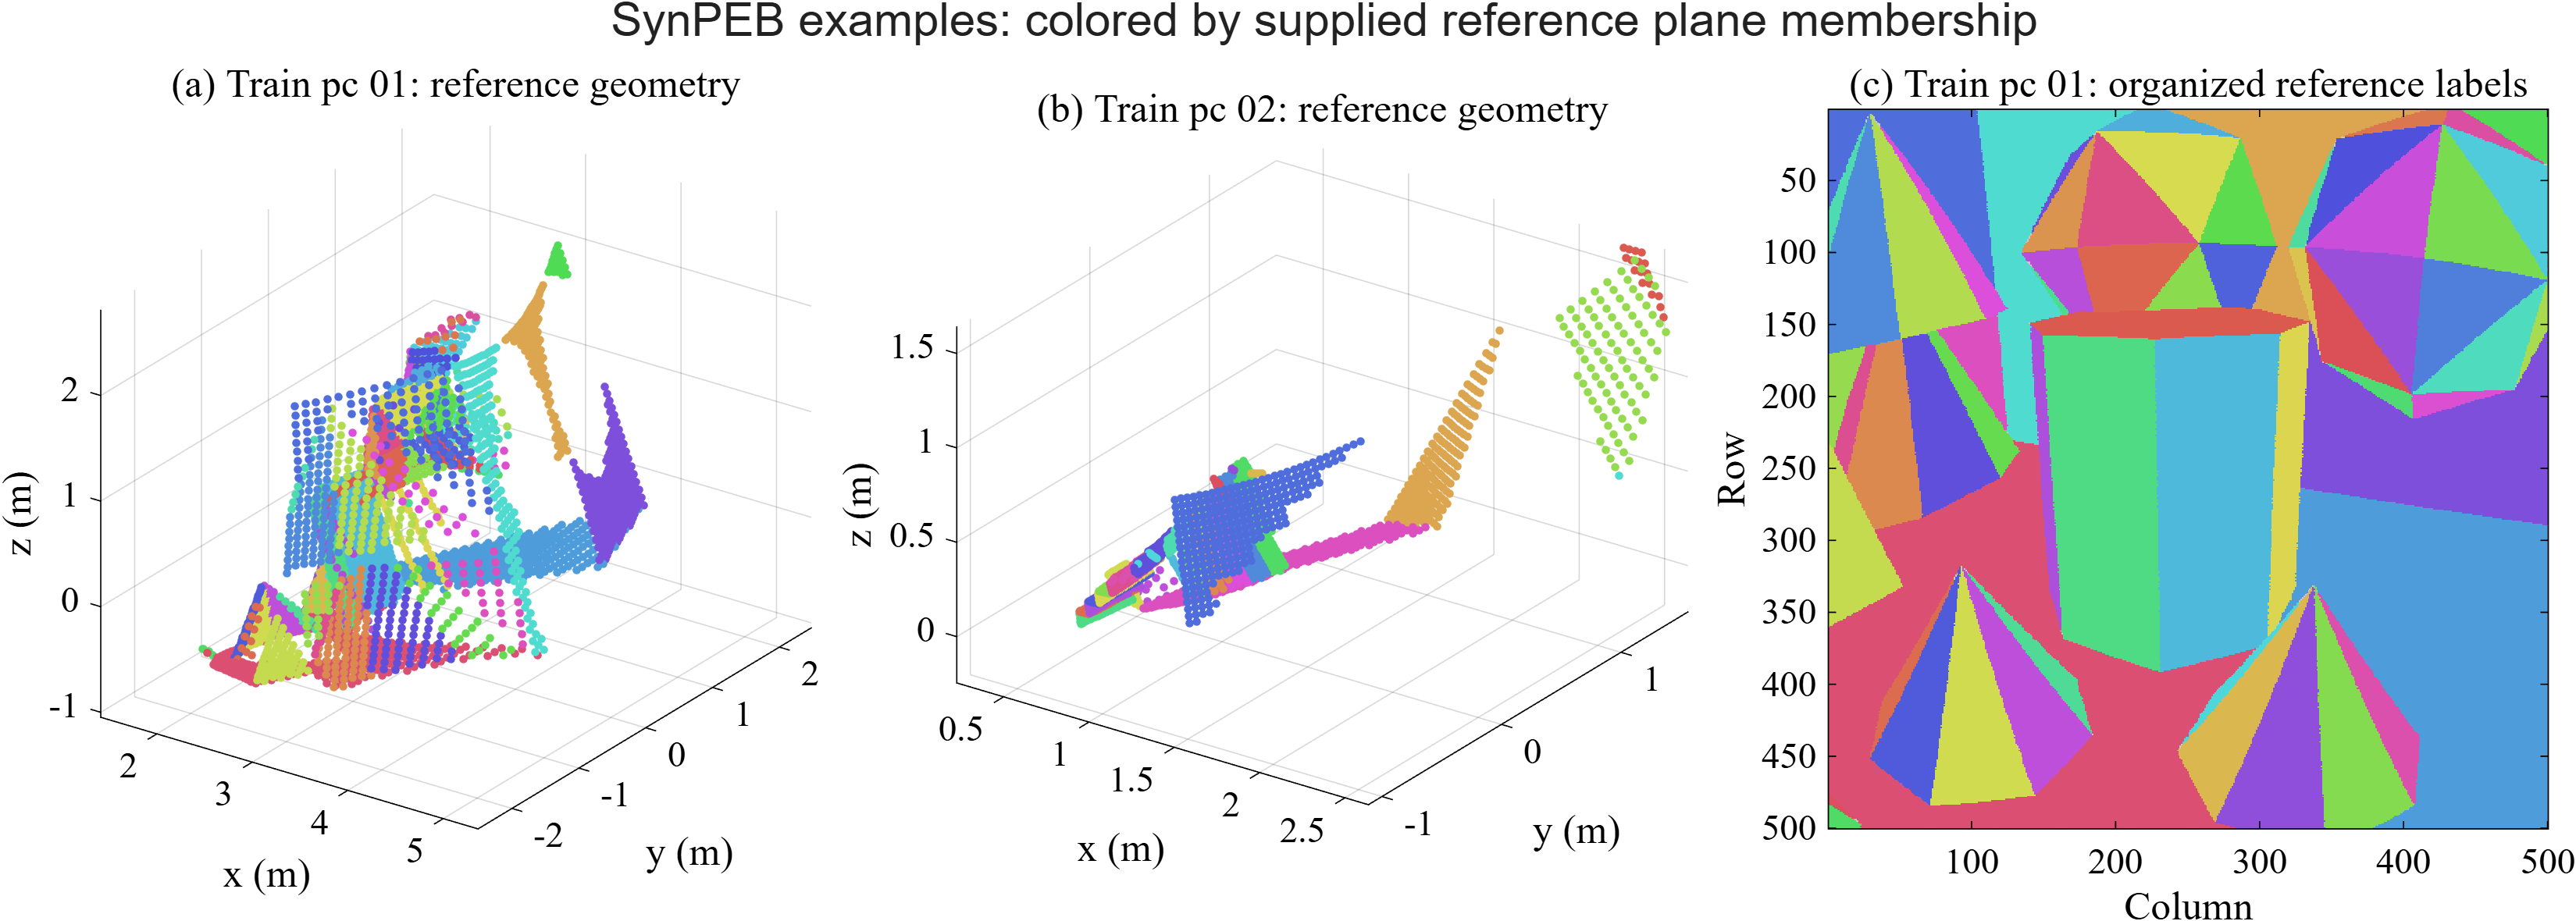
\includegraphics[width=\textwidth]{figures/dataset_overview.png}
\caption{Fixed training examples. Panels (a) and (b) show reference geometry from gt/pc\_01 and gt/pc\_02 at the experimental stride of eight; (c) shows the full-resolution organized label map of gt/pc\_01. Colors denote the supplied plane memberships within each scan and carry no semantic meaning. They are visualization annotations, not algorithm inputs.}
\label{fig:dataset_overview}
\end{figure*}

\begin{figure*}[!t]
\centering
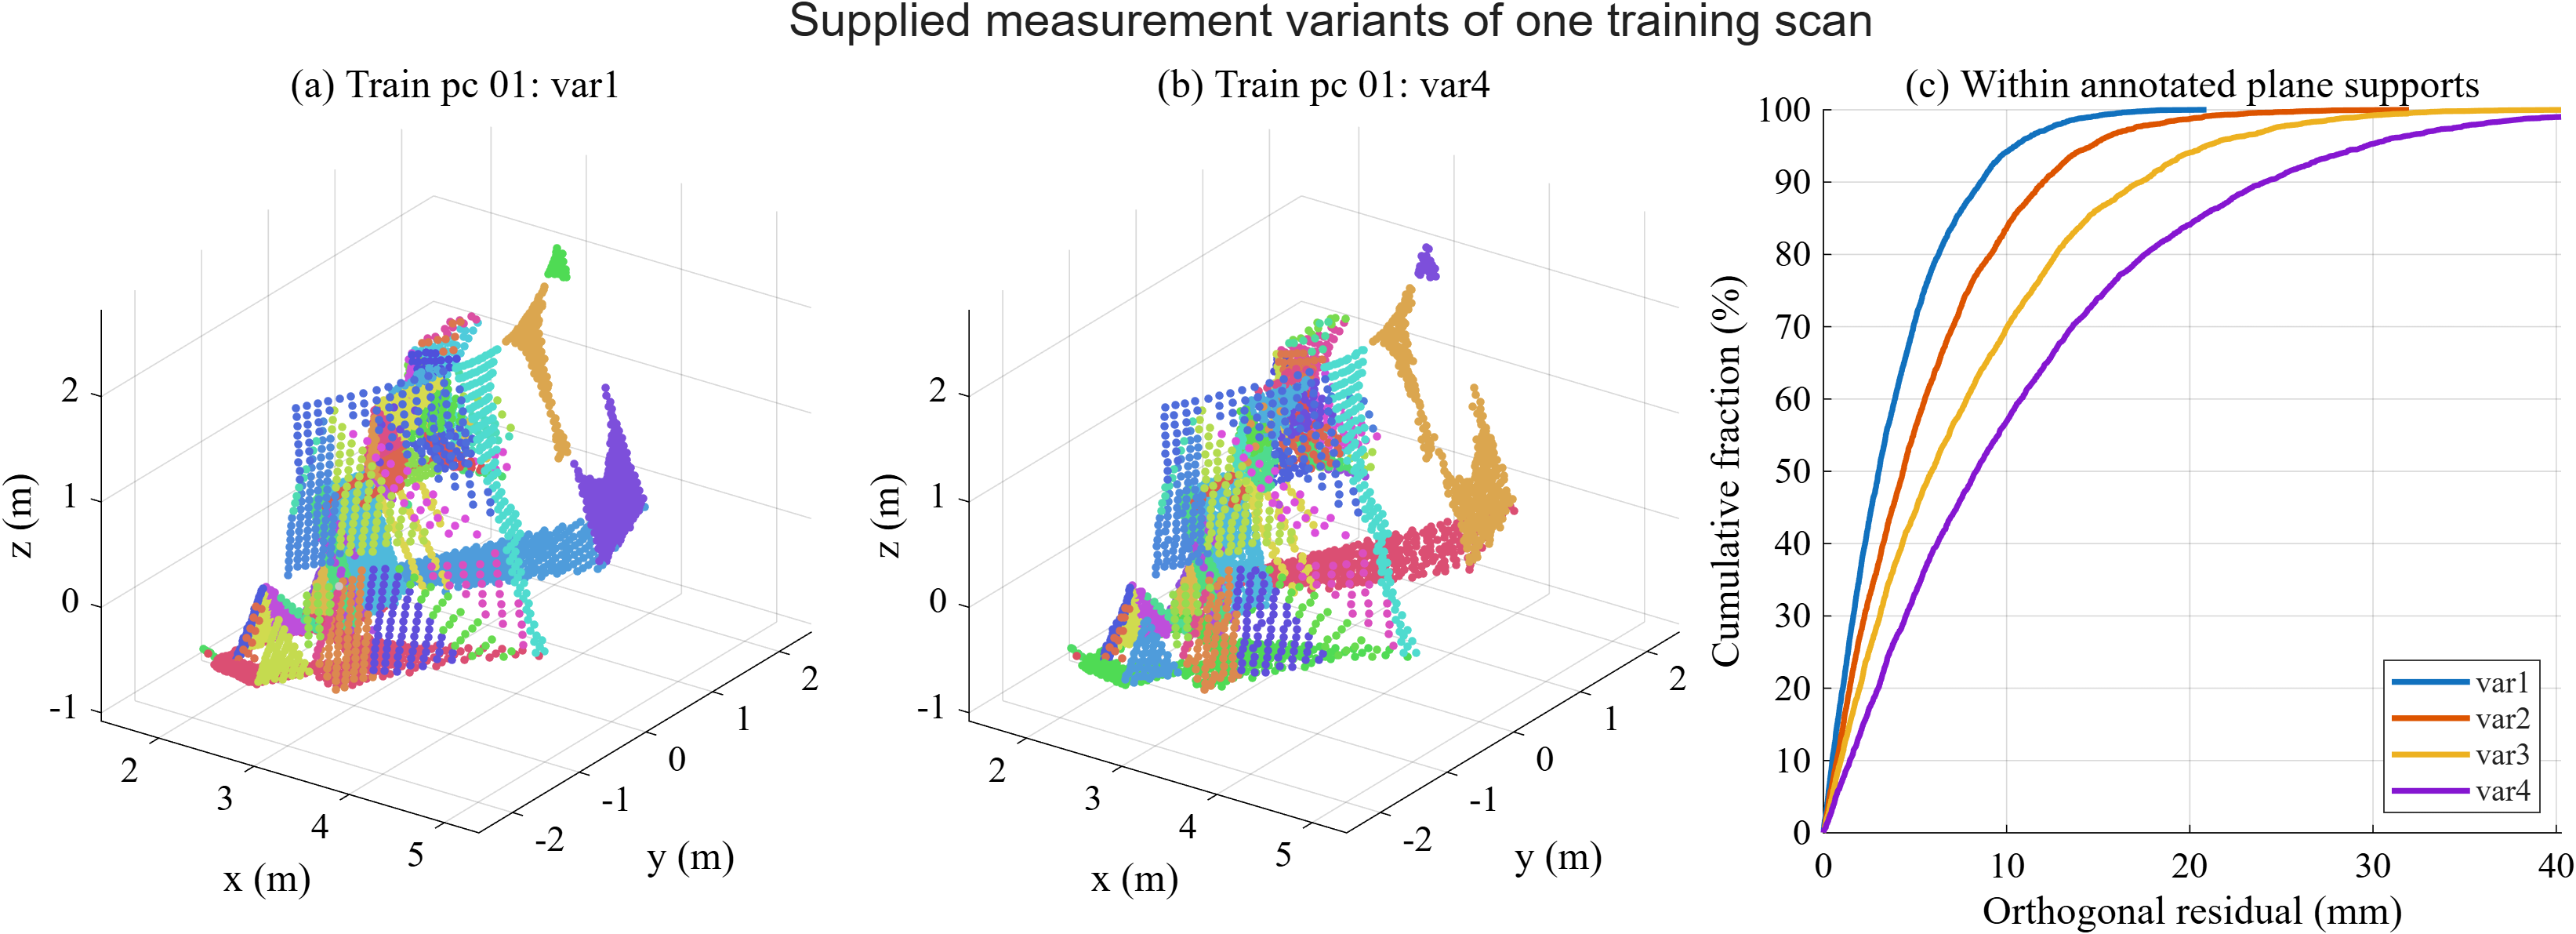
\includegraphics[width=\textwidth]{figures/dataset_variants.png}
\caption{Measurement variants of training scan pc\_01. Panels (a) and (b) use the same view and axis limits, with each file colored using its own annotations. Panel (c) shows cumulative orthogonal residuals after fitting planes to each variant's annotated supports at stride eight. This is a descriptive geometric diagnostic, not an algorithm result or a calibrated estimate of sensor noise. The horizontal range ends at the largest variant-specific 99th percentile; all valid residuals enter each cumulative fraction. Degenerate annotated supports are omitted from this diagnostic.}
\label{fig:dataset_variants}
\end{figure*}

\subsection{Preprocessing and spatial graph}\label{preprocessing-and-spatial-graph}

Point ordering is preserved when decoding the PCD files. The organized row--column index is converted to the corresponding point index before sampling. Every eighth row and column is retained, starting from index one. For a complete 500 \(\times\) 500 scan, this produces 63 \(\times\) 63 = 3,969 points, approximately 1.59\% of the original measurements. Non-finite coordinates and all-zero coordinate records are discarded after sampling. Reference labels follow exactly the same retained indices.

The corresponding variant's own intensity labels provide the evaluation reference; labels are not copied blindly from a same-named gt file. This preserves consistency between the measured coordinates and their supplied annotations. Points excluded by the evaluation mask can still participate in fitting and spatial optimization. The ground-truth mask is not used to select hypotheses, construct neighborhoods, or remove input points.

The PEARL graph joins horizontally and vertically adjacent valid sampled positions, removing edges longer than 0.30 m. Remaining edge weights are \(\exp(-\|x_i-x_j\|_2^2/(2\sigma^2))\), with \(\sigma\) = 0.15 m. For the Fig.~\ref{fig:dataset_preprocessing} example, the graph contains 3,969 nodes and 7,412 edges. Colors in the graph illustration reveal reference supports, while connectivity is computed entirely from geometry. All compared methods use the same sampled cloud; the two PEARL pipelines use the same graph.

\begin{figure*}[!t]
\centering
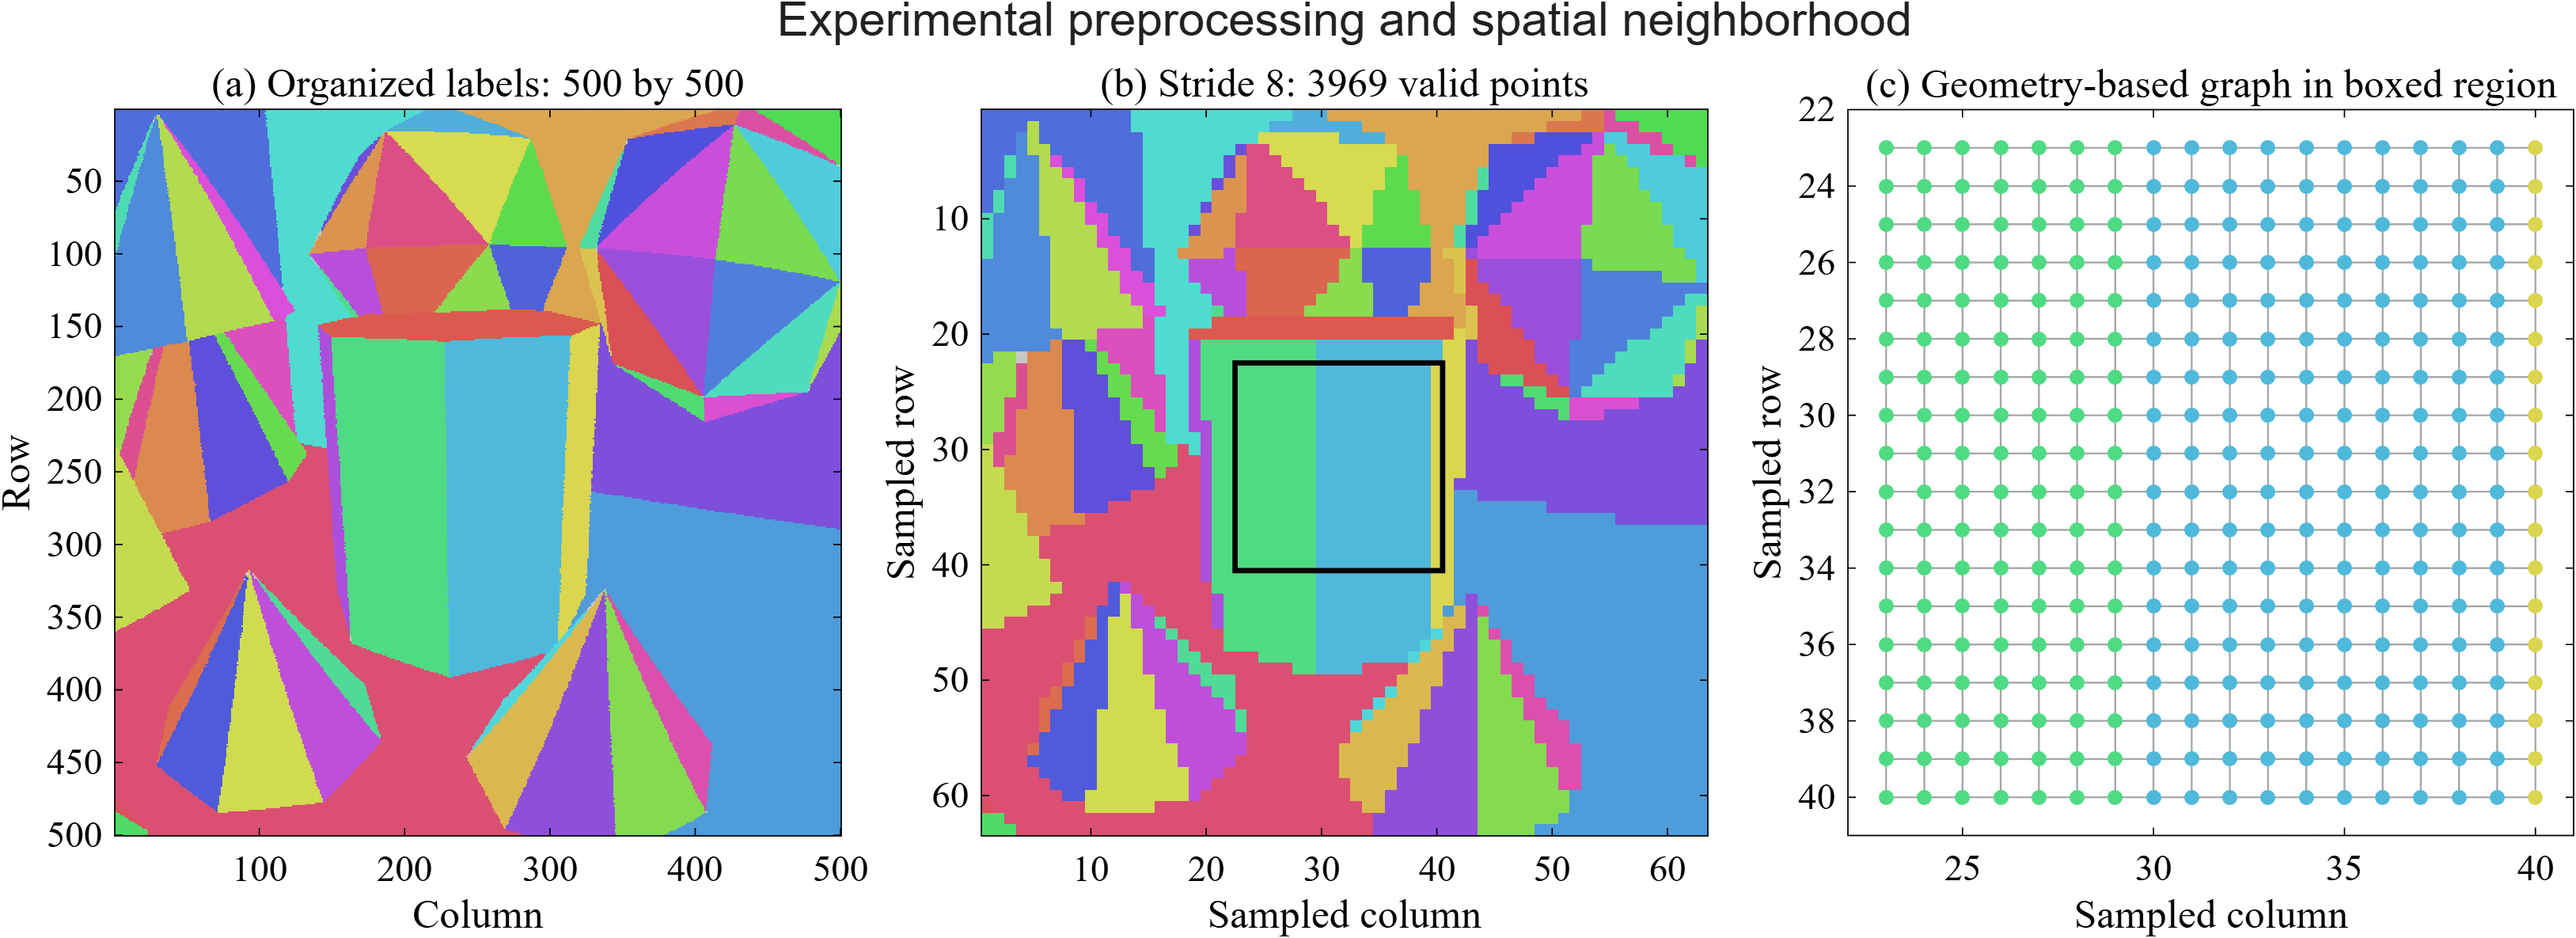
\includegraphics[width=\textwidth]{figures/dataset_preprocessing.png}
\caption{Preprocessing of train/var1/pc\_01. (a) Original organized reference map. (b) The stride-eight grid, with the magnified region boxed. (c) Retained horizontal and vertical neighborhood edges within that region. Edge construction uses grid adjacency and three-dimensional separation, without reference IDs. The annotations are overlaid solely to make the graph's relation to surfaces visible.}
\label{fig:dataset_preprocessing}
\end{figure*}

\subsection{Parameter selection and test protocol}\label{parameter-selection-and-test-protocol}

The training split is used to select hyperparameters, not to learn reusable plane coefficients or classifier weights. Screening evaluates scans 1--2, variants var1 and var4, and seed 7. A staged search varies proposal count, plane cap, and local sampling radius, then examines 25 distance-threshold and smoothness-ratio combinations, followed by minimum support. Previously evaluated configurations are reused. This is a heuristic staged search rather than an exhaustive search over the full parameter product.

The three highest-ranked screened configurations are confirmed on the disjoint training scans 3--10, all four variants, and seeds 7, 19, and 43. This gives 96 scan--variant--seed records per configuration and method. Ranking maximizes the equally weighted average of RANSAC and PEARL mean matched Intersection over Union (IoU; see Section~\ref{evaluation-metrics}); ties use the corresponding mean F1 score (see Section~\ref{evaluation-metrics}), then summed mean runtime. This selection criterion is shared across the two methods, rather than optimized for PEARL accuracy alone.

The confirmed configuration uses 1,000 PEARL proposal attempts, a plane cap of 150, minimum support six, local radius eight, distance threshold 0.04 m, and smoothness ratio 0.4. PEARL permits 15 outer iterations and three expansion sweeps per iteration; the remaining settings follow Sections~\ref{ransac-and-sequential-ransac}--\ref{hybrid-ransac-and-pearl-method}. These values are frozen before testing. The hybrid uses the same settings without separate tuning.

Final testing covers 30 scans \(\times\) 4 variants \(\times\) 3 seeds = 360 records per method. Resetting the generator before each pipeline makes each scan--variant--seed case reproducible. The three methods are evaluated on identical input points. The hybrid starts from the exact standalone RANSAC result, and the no-smoothness ablation uses the sampled PEARL plane bank with the smoothness ratio set to zero. Repeated seeds and variants are correlated; reported means and standard deviations are descriptive across records rather than uncertainty estimates from 360 independent scenes.

\subsection{Evaluation metrics}\label{evaluation-metrics}

Predicted plane numbers have no intrinsic relation to the reference numbers. Let V denote the indices with evaluable reference labels, \(G_{a}\) the support of reference plane a, and \(S_{b}\) the support of predicted plane b restricted to V. Predicted label zero is excluded from the predicted-plane set and denotes rejection. The overlap matrix is

\begin{equation}
C_{ab}=|G_a\cap S_b|.
\label{eq:57}
\end{equation}

A partial one-to-one matching \(\pi\) between reference and predicted planes maximizes total overlap:

\begin{equation}
\pi^*\in\operatorname*{arg\,max}_{\pi}\sum_{(a,b)\in\pi}C_{ab}.
\label{eq:58}
\end{equation}

Matched point accuracy is the fraction of evaluable points assigned to their matched reference plane:

\begin{equation}
\mathrm{Accuracy}=\frac{\sum_{(a,b)\in\pi^*}C_{ab}}{|V|}.
\label{eq:59}
\end{equation}

Rejected reference-plane points and points assigned to unmatched predicted planes count as errors. Unlike many-to-one matching, this rule does not allow several fragments of one reference plane to all receive correct labels. Confusion matrices are computed after matching and saved per case, since plane IDs are scan-specific. Row-normalized displays show within-reference-plane assignment proportions; they do not replace the count-based accuracy calculation.

Intersection over Union (IoU) measures how closely a predicted plane's points match those of a reference plane. It divides the number of evaluable points in both planes (the intersection) by the number in either plane (the union). IoU ranges from 0 for no shared points to 1 for identical point sets. For example, if a reference plane contains 80 points and a predicted plane contains 70 evaluable points, with 60 shared points, their IoU is 60 / (80 + 70 \(-\) 60) \(\approx\) 0.67. For a reference--prediction pair,

\begin{equation}
\mathrm{IoU}_{ab}=\frac{C_{ab}}{|G_a|+|S_b|-C_{ab}}.
\label{eq:60}
\end{equation}

Mean matched IoU uses the same maximum-overlap matching as point accuracy, rather than a matching that directly maximizes IoU:

\begin{equation}
\mathrm{mIoU}=\frac1G\sum_{(a,b)\in\pi^*}\mathrm{IoU}_{ab}.
\label{eq:61}
\end{equation}

Here G is the total number of evaluable reference planes, so unmatched reference planes contribute zero. This macro-average gives each reference plane equal weight, whereas point accuracy gives large supports greater influence. In the saved test cases, the 120 distinct scan--variant inputs contain 9--88 reference planes after sampling, with a mean of 40.93; these counts are not multiplied by the repeated seeds.

Plane-instance detection uses a separate one-to-one matching restricted to pairs with IoU \(\geq\) 0.5. The implementation assigns each eligible edge weight 1 + IoU and maximizes the sum of those weights; accepted pairs define true positives TP. Recall is the fraction of evaluable reference planes that are successfully matched (TP out of G). Precision is the fraction of extracted planes that are successfully matched (TP out of B, where B counts all extracted positive-label planes). The F1 score is the harmonic mean of precision and recall: it is high only when both are high. The three metrics are calculated as follows:

\begin{equation}
\mathrm{Precision}=\frac{\mathrm{TP}}B,\qquad\mathrm{Recall}=\frac{\mathrm{TP}}G,
\label{eq:62}
\end{equation}

\begin{equation}
F_1=\frac{2\,\mathrm{Precision}\,\mathrm{Recall}}{\mathrm{Precision}+\mathrm{Recall}}.
\label{eq:63}
\end{equation}

For example, if 6 of 10 evaluable reference planes are matched and 8 planes were extracted, recall is 6/10 = 0.60 and precision is 6/8 = 0.75, giving an F1 score of about 0.67. Zero denominators are handled explicitly in the implementation. All extracted planes enter B, including planes supported only by ignored points; such a plane cannot match an evaluable reference. A missed plane is an unmatched reference under the detection matching, giving G \(-\) TP. Point errors, mean matched IoU, and instance detection therefore measure different aspects of segmentation quality.

Oversegmentation counts reference planes for which at least two predictions each cover 10\% or more of the reference support. Undersegmentation counts predictions for which at least two reference planes each constitute 10\% or more of their evaluable support. These are project-specific diagnostic definitions and are not assumed identical to the original SynPEB paper's evaluation protocol. The number of extracted planes is also reported.

Algorithm timers exclude data loading, graph construction, reference matching, and figure export. Hybrid total time includes RANSAC initialization once plus PEARL refinement; component times are recorded separately. PEARL histories report the original geometric-plus-spatial energy after initialization, expansion, and refitting. Energy descent verifies progress on the chosen objective but does not by itself establish improved reference accuracy. Mean accuracy across records and point-weighted aggregate accuracy are reported separately.

\subsection{Dataset limitations and scope}\label{dataset-limitations-and-scope}

SynPEB supplies controlled geometric annotations, but its synthetic polyhedral environment does not cover the full diversity of real sensors, material effects, dynamic objects, curved surfaces, and clutter. Performance on these scans therefore supports conclusions about this benchmark and configuration, rather than general real-world robustness. The graph also assumes an organized scan, which limits direct transfer to arbitrary unorganized point clouds.

Stride-eight sampling reduces computational cost while removing small supports and altering neighborhood distances. The number of remaining annotated planes can differ from the original full-resolution count. Results must therefore be compared under the same sampling policy. In addition, finite reference patches are evaluated against models of infinite planes: touching or coplanar regions may be geometrically ambiguous without extra appearance or object information.

Stanford S3DIS \cite{armeni2016s3dis} offers real indoor scans annotated for semantic building elements and objects. These annotations do not directly define a complete plane-instance partition: one object may contain several planar faces, and one semantic class may span many distinct planes. Additional geometric annotation would be needed for the same plane-level matching protocol. SynPEB was chosen to make reference plane membership explicit, while a separately annotated real-data evaluation remains a useful extension.

\section{Results and Discussion}\label{results-and-discussion}

The completed test experiments show a clear accuracy--runtime tradeoff. Sampled-proposal PEARL achieves the strongest point accuracy and reference-plane overlap, sequential RANSAC is fastest, and the hybrid improves the RANSAC segmentation at intermediate cost. Removing spatial regularization causes a large loss of segmentation quality in the selected PEARL configuration. All summaries below use the saved per-case measurements and predictions, with 360 scan--variant--seed records per method; no segmentation was rerun to produce these figures.

\subsection{Three way segmentation comparison}\label{three-way-segmentation-comparison}

Table~\ref{tab:comparison} and Fig.~\ref{fig:results_three_way} compare the three pipelines under the frozen parameter configuration. Sampled PEARL attains 84.26\% mean matched point accuracy, compared with 69.89\% for RANSAC and 77.98\% for the hybrid. Its gain over RANSAC is 14.37 percentage points, or 20.56\% relative to the baseline accuracy. The hybrid gains 8.08 percentage points, or 11.56\% relative. Point-weighted accuracies are nearly identical to the corresponding record means, consistent with the common sampling policy.

The same ordering holds for mean matched IoU and F-score. Sampled PEARL increases mean matched IoU from 0.2086 to 0.4554, a relative improvement of 118.26\%; the hybrid reaches 0.2836, a 35.91\% relative improvement. These plane-weighted scores are substantially lower than point accuracy because recovering a large support does not compensate for missing many smaller reference planes. The aggregate accuracy ordering is unchanged across the three seeds; their method-specific aggregate means span less than 0.5 percentage points. This does not imply that individual cases are insensitive to initialization.

\begin{table*}[!t]
\caption{Three-way comparison on 360 test records per method. Accuracy is mean \(\pm\) descriptive standard deviation; these are correlated records, not independent samples. Mean matched IoU and F-score follow Section~\ref{dataset-and-experimental-setup}. Runtime comes from the initialization-comparison run only.}
\label{tab:comparison}
\centering\footnotesize
\begin{tabular}{lrrrr}
\hline
\shortstack{Method} & \shortstack{Accuracy\\(\%)} & \shortstack{Matched\\IoU} & \shortstack{F-score} & \shortstack{Total\\time\\(s)} \\ \hline
RANSAC & 69.89 \(\pm\) 9.74 & 0.2086 & 0.2257 & 0.376 \\
Sampled PEARL & 84.26 \(\pm\) 8.31 & 0.4554 & 0.4003 & 19.620 \\
Hybrid & 77.98 \(\pm\) 9.47 & 0.2836 & 0.3443 & 2.512 \\
\hline
\end{tabular}
\end{table*}

\begin{figure*}[!t]
\centering
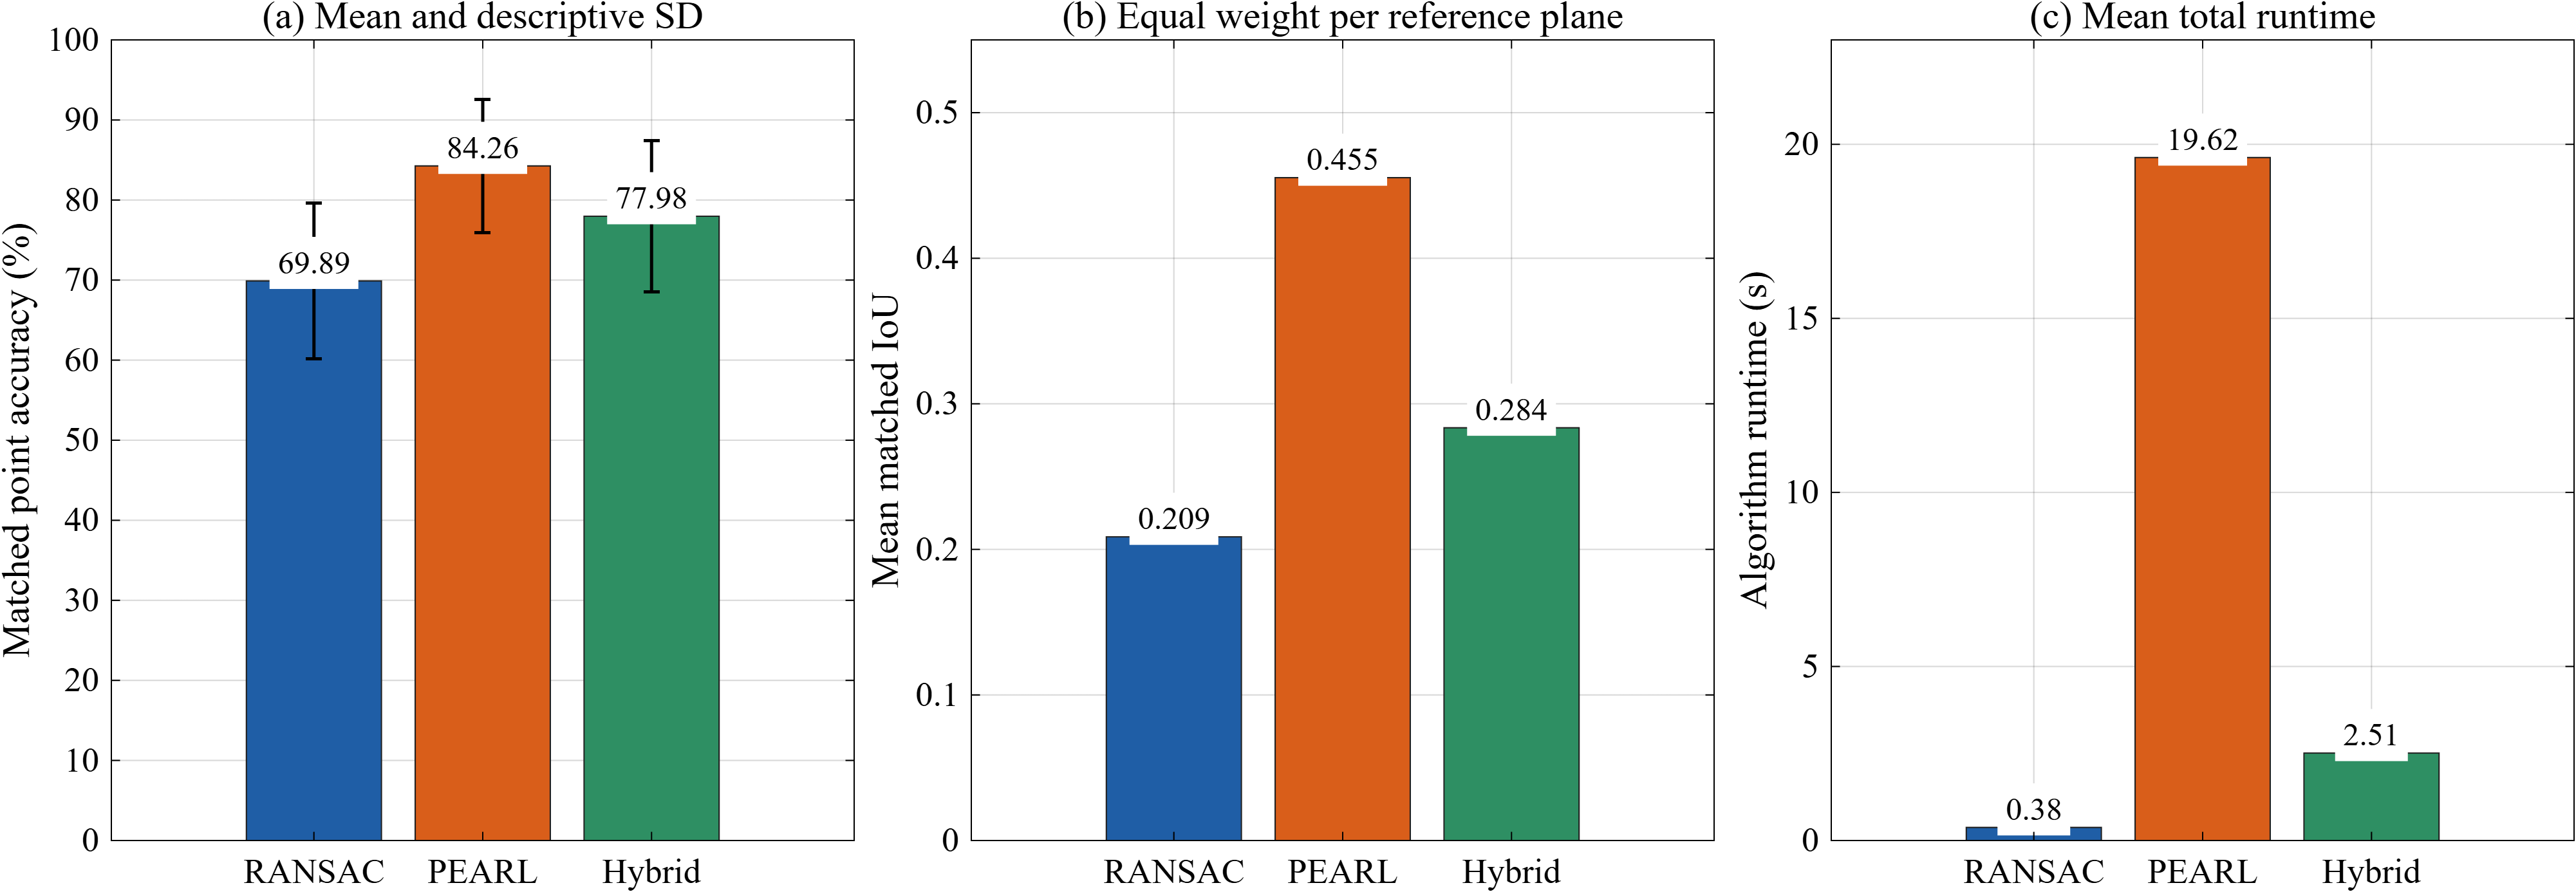
\includegraphics[width=\textwidth]{figures/results_three_way.png}
\caption{Accuracy, reference-plane overlap, and algorithm runtime from the same three-way comparison run. PEARL denotes the sampled-proposal pipeline. Error bars in (a) show descriptive variation across records and are not confidence intervals. The hybrid includes the cost of its RANSAC initialization.}
\label{fig:results_three_way}
\end{figure*}

\subsection{Computational cost and model bank size}\label{computational-cost-and-model-bank-size}

RANSAC requires 0.376 s per record on average, the hybrid 2.512 s, and sampled PEARL 19.620 s. The hybrid is about 7.81 times faster than sampled PEARL, while retaining lower accuracy and overlap; it remains 6.68 times slower than standalone RANSAC. Sampled PEARL costs about 52.20 times the RANSAC runtime in this run. These ratios describe the MATLAB implementations and selected settings, rather than intrinsic complexity constants of the algorithms.

Table~\ref{tab:components} separates initialization from refinement. Sampled PEARL generates its proposal bank in only 0.135 s, whereas RANSAC initialization requires 0.376 s. The hybrid's runtime advantage therefore comes from the subsequent refinement stage rather than a faster initializer. Its mean refinement time is 2.137 s, compared with 19.484 s for sampled PEARL. The smaller model bank is consistent with this difference: the hybrid begins with 19.12 planes on average, while sampled PEARL begins with 150. Each expansion sweep visits every available label, making bank size relevant to graph-cut workload. The experiment does not independently control bank size to establish it as the sole cause.

\begin{table*}[!t]
\caption{Mean model counts and runtime components. ``At cap'' counts records that complete all 15 outer iterations, out of 360. The reference contains 40.93 planes per sampled scan--variant input on average. RANSAC has no PEARL iteration count.}
\label{tab:components}
\centering\footnotesize
\begin{tabular}{lrrrrr}
\hline
\shortstack{Method} & \shortstack{Initial\\planes} & \shortstack{Final\\planes} & \shortstack{Init.\\time\\(s)} & \shortstack{Refine\\time\\(s)} & \shortstack{At\\cap} \\ \hline
RANSAC & 19.12 & 19.12 & 0.376 & 0.000 & --- \\
Sampled PEARL & 150.00 & 54.25 & 0.135 & 19.484 & 89 \\
Hybrid & 19.12 & 19.09 & 0.376 & 2.137 & 60 \\
\hline
\end{tabular}
\end{table*}

The hybrid finishes with 19.09 planes on average and cannot add labels beyond its RANSAC bank. Its mean instance precision is 0.4903, greater than sampled PEARL's 0.3776, but its recall is lower, 0.2743 versus 0.4501. This is consistent with a smaller collection of detected planes that leaves more reference structures unrecovered. Sampled PEARL ends with 54.25 planes on average, showing that unused labels are removed, although this does not guarantee the correct model count. The iteration cap is reached in 89 sampled-PEARL records and 60 hybrid records. Further energy reduction may therefore be possible in some cases, without a guarantee of higher accuracy.

\subsection{Paired refinement and energy reduction}\label{paired-refinement-and-energy-reduction}

Starting from the exact RANSAC output, the hybrid improves point accuracy in 357 of 360 records and reduces it in three; there are no ties at the reporting tolerance. Mean matched IoU increases by 0.0749 and mean F-score by 0.1187. Independently recomputed energy does not increase in any paired case, and its mean decrease is 0.5041 in the original squared-distance units. Fig.~\ref{fig:results_paired_energy} distinguishes this optimization behavior from reference-label accuracy.

\begin{figure*}[!t]
\centering
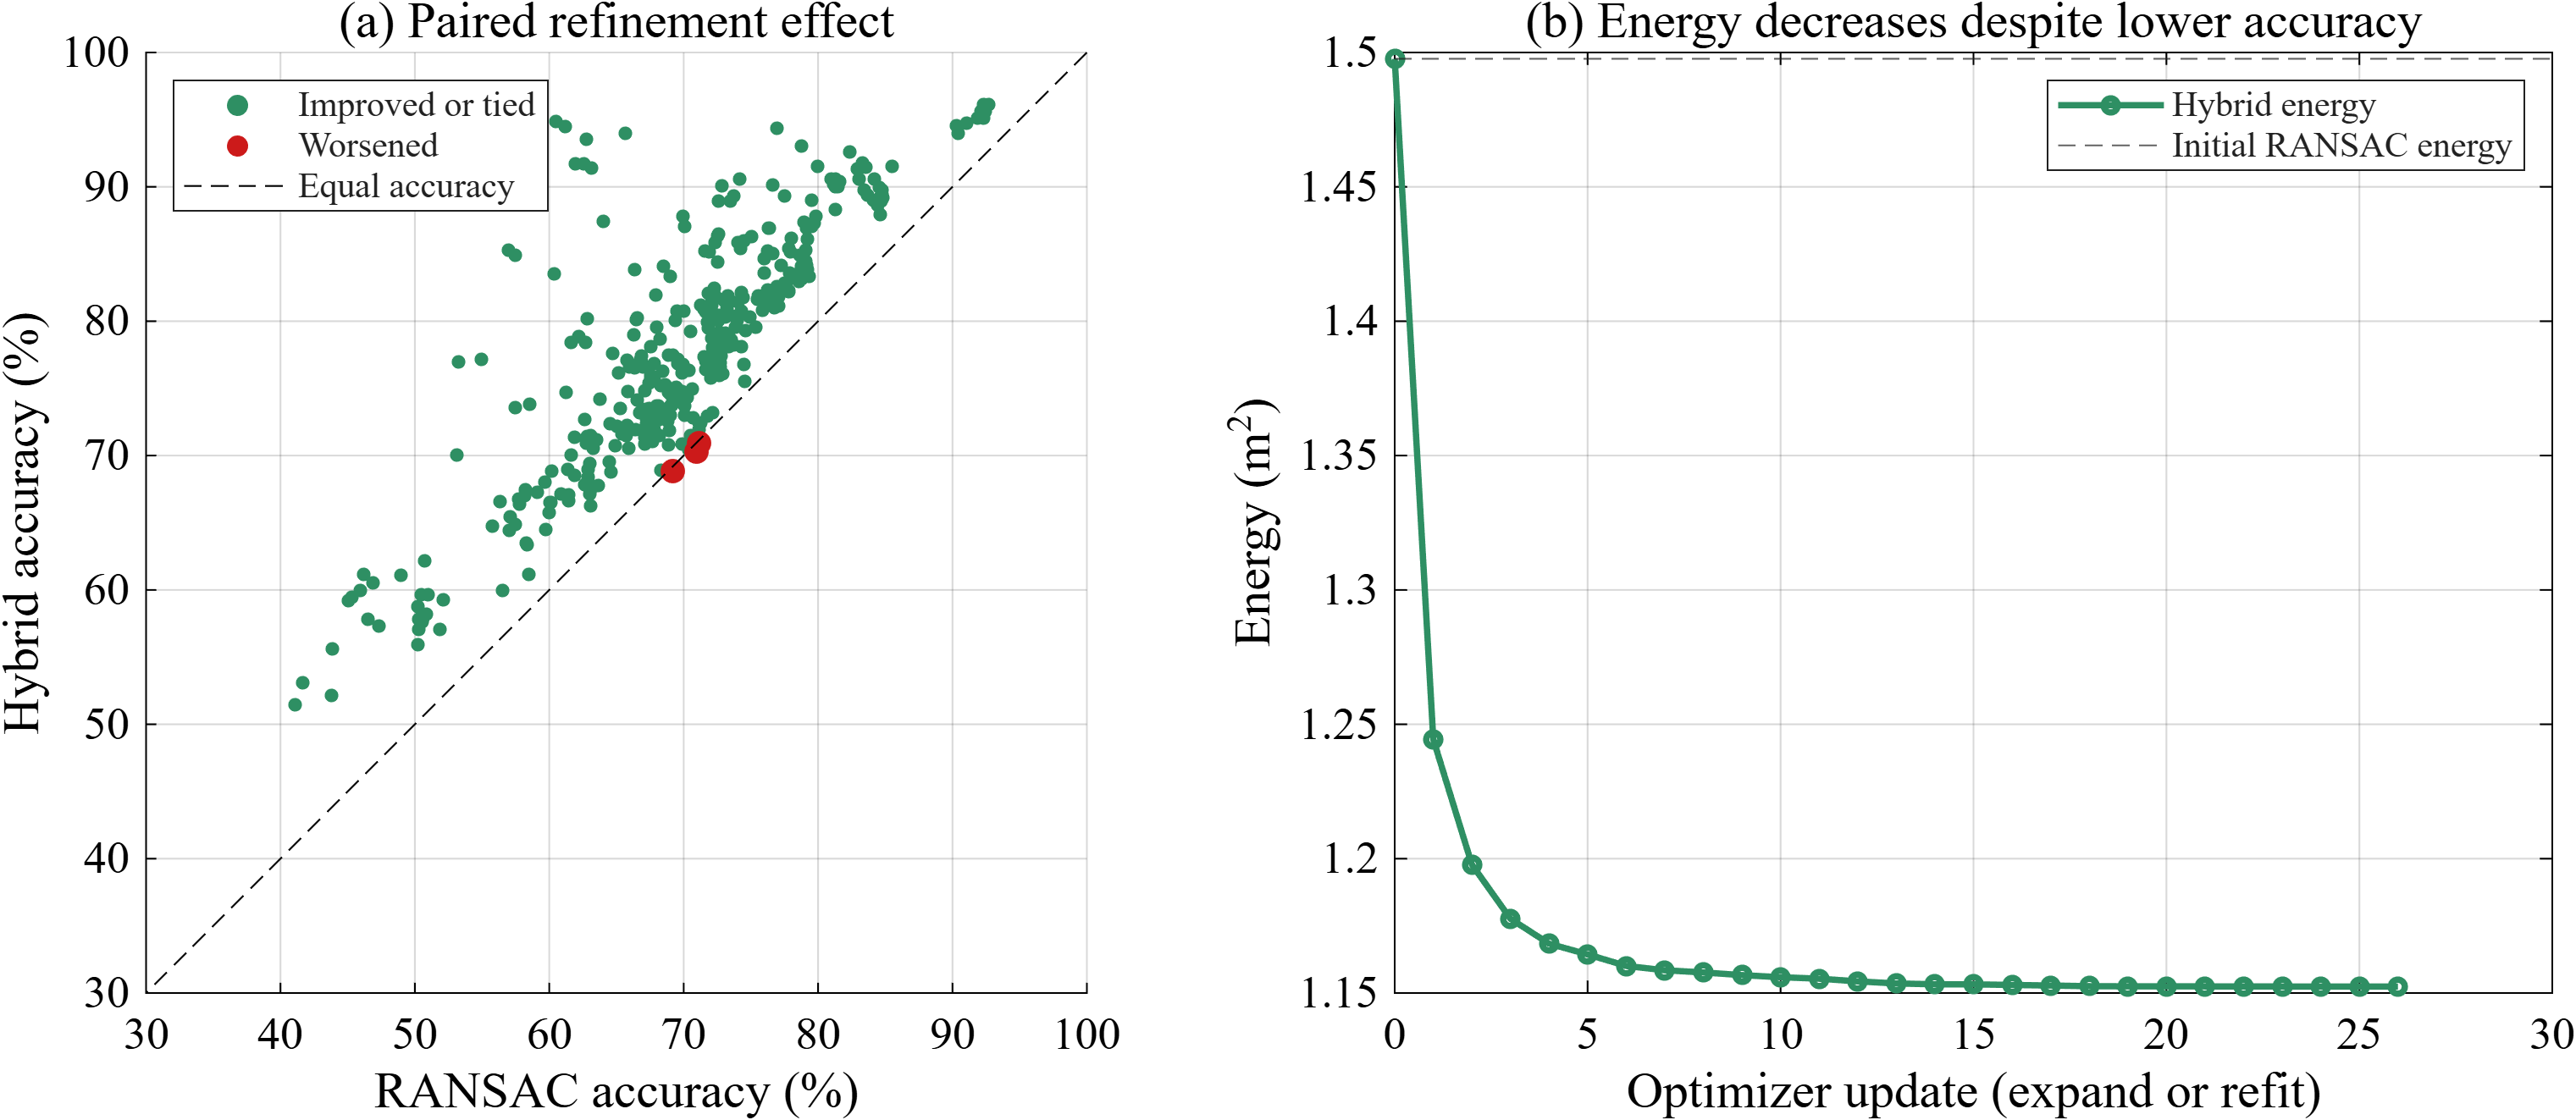
\includegraphics[width=\textwidth]{figures/results_paired_energy.png}
\caption{(a) Paired point accuracies for all 360 RANSAC and hybrid records; red markers identify the three decreases. (b) Hybrid energy history for test pc\_25, var1, seed 19, the largest accuracy regression. Energy decreases from 1.4977 to 1.1524 even though accuracy falls from 70.97\% to 70.26\%. Updates alternate expansion and refitting; the plot does not imply that intermediate accuracy was measured.}
\label{fig:results_paired_energy}
\end{figure*}

\subsection{Poorly segmented examples}\label{poorly-segmented-examples}

Fig.~\ref{fig:results_failure_cases} deliberately shows failure cases rather than visually favorable examples. The first is the scan--variant case with the lowest three-method mean point accuracy among seed-7 records. The second is the largest hybrid accuracy regression across all 360 paired records. These criteria make the selection reproducible, while the examples are not intended to estimate the prevalence of a failure pattern.

For test pc\_03, var4, seed 7, RANSAC achieves 41.63\% accuracy, sampled PEARL 64.52\%, and the hybrid 53.08\%. Matched IoUs are 0.1006, 0.2599, and 0.1518, respectively. The reference contains 57 planes, compared with 25, 77, and 25 extracted planes. The maps expose disagreement along boundaries and small supports. Sampled PEARL improves the segmentation but still leaves substantial plane-level errors; increased point accuracy should not be interpreted as complete structure recovery.

For test pc\_25, var1, seed 19, RANSAC accuracy falls from 70.97\% to 70.26\% after refinement, while matched IoU rises slightly from 0.0686 to 0.0716. Energy decreases by 0.3452. Thus, the optimizer improves its chosen objective and one overlap measure while worsening another evaluation measure. Both RANSAC and the hybrid return 17 planes for 69 reference planes. Sampled PEARL returns 92 planes and reaches 79.01\% accuracy, but its matched IoU remains only 0.2362. A good fit to large supports can coexist with many missed, merged, or fragmented smaller structures.

\begin{figure*}[!t]
\centering
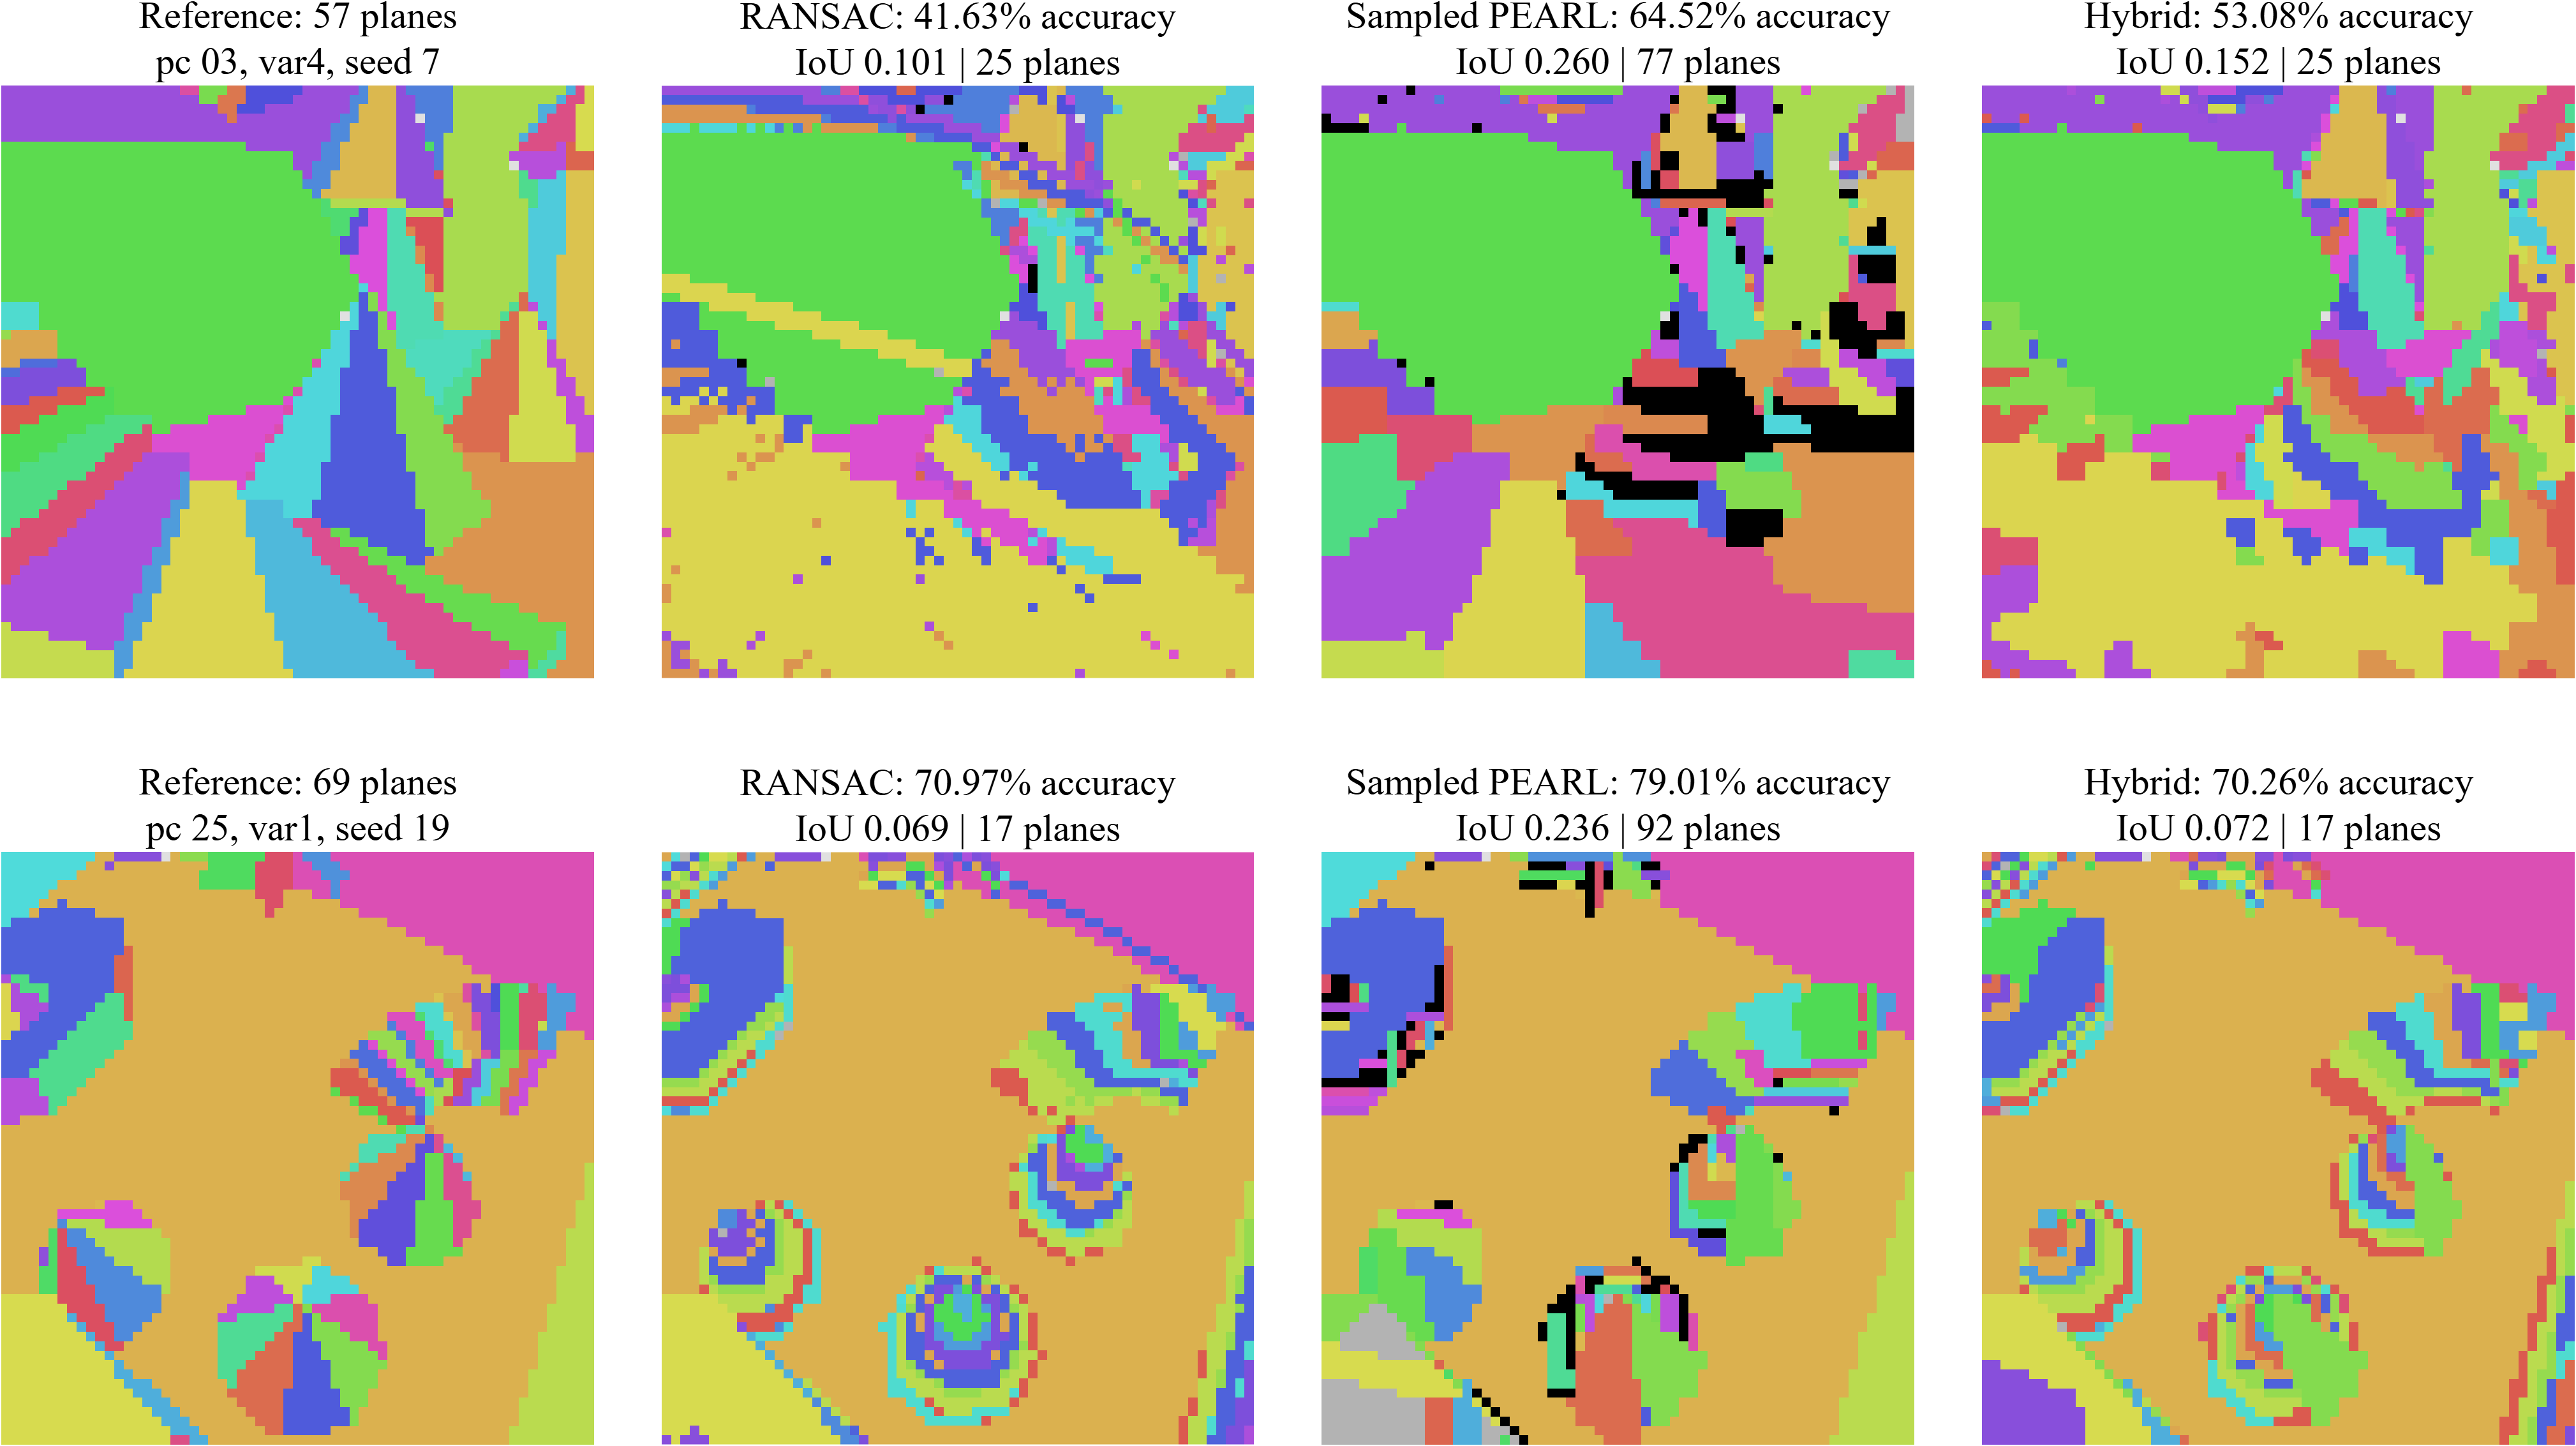
\includegraphics[width=\textwidth]{figures/results_failure_cases.png}
\caption{Saved predictions for the two explicitly selected difficult cases. Each row shows reference labels, RANSAC, sampled PEARL, and the hybrid on the organized stride-eight grid. Colors are aligned independently in each row by the same one-to-one matching used for evaluation. Black denotes an unmatched predicted plane, gray denotes rejection, and light gray denotes ignored reference points. A matched color identifies the mapped plane, not a guarantee that every point of that color is correct. Titles report point accuracy, mean matched IoU, and plane count.}
\label{fig:results_failure_cases}
\end{figure*}

\subsection{Spatial regularization ablation}\label{spatial-regularization-ablation}

The ablation compares sampled PEARL at \(\eta\) = 0.4 with the same pipeline at \(\eta\) = 0. Both conditions use the same input points, initial plane bank, data-cost scaling, and iteration budgets. Plane parameters are still re-estimated by SVD when the spatial term is removed. This is a test of spatial coupling under a fixed selected configuration, not a comparison with absent training or missing initialization. The generator is reset, but label-visit orders are not explicitly matched because the ablation skips proposal generation.

Table~\ref{tab:ablation} shows that mean accuracy falls from 84.26\% to 11.27\%, a decrease of 72.99 percentage points. Mean matched IoU falls from 0.4554 to 0.0746, and mean F-score from 0.4003 to 0.0005. The spatial-prior condition has greater accuracy and matched IoU in every paired record. Without the prior, all 150 candidate labels remain active in every case, compared with 54.25 active labels on average when regularization is present. The observed scattered assignments and retained label count are consistent with the lack of a penalty for spatial disagreement or model count in the unregularized objective.

\begin{table*}[!t]
\caption{Spatial-prior ablation over 360 records per condition. Runtime is measured within the separate ablation run and must not be mixed with the timing values in Table~\ref{tab:comparison}. Accuracy and overlap of the regularized condition reproduce the three-way comparison exactly.}
\label{tab:ablation}
\centering\footnotesize
\begin{tabular}{lrrrrr}
\hline
\shortstack{Condition} & \shortstack{Accuracy\\(\%)} & \shortstack{Matched\\IoU} & \shortstack{F-score} & \shortstack{Final\\planes} & \shortstack{Time\\(s)} \\ \hline
\(\eta\) = 0.4 & 84.26 \(\pm\) 8.31 & 0.4554 & 0.4003 & 54.25 & 36.497 \\
\(\eta\) = 0 & 11.27 \(\pm\) 3.76 & 0.0746 & 0.0005 & 150.00 & 27.526 \\
\hline
\end{tabular}
\end{table*}

\begin{figure*}[!t]
\centering
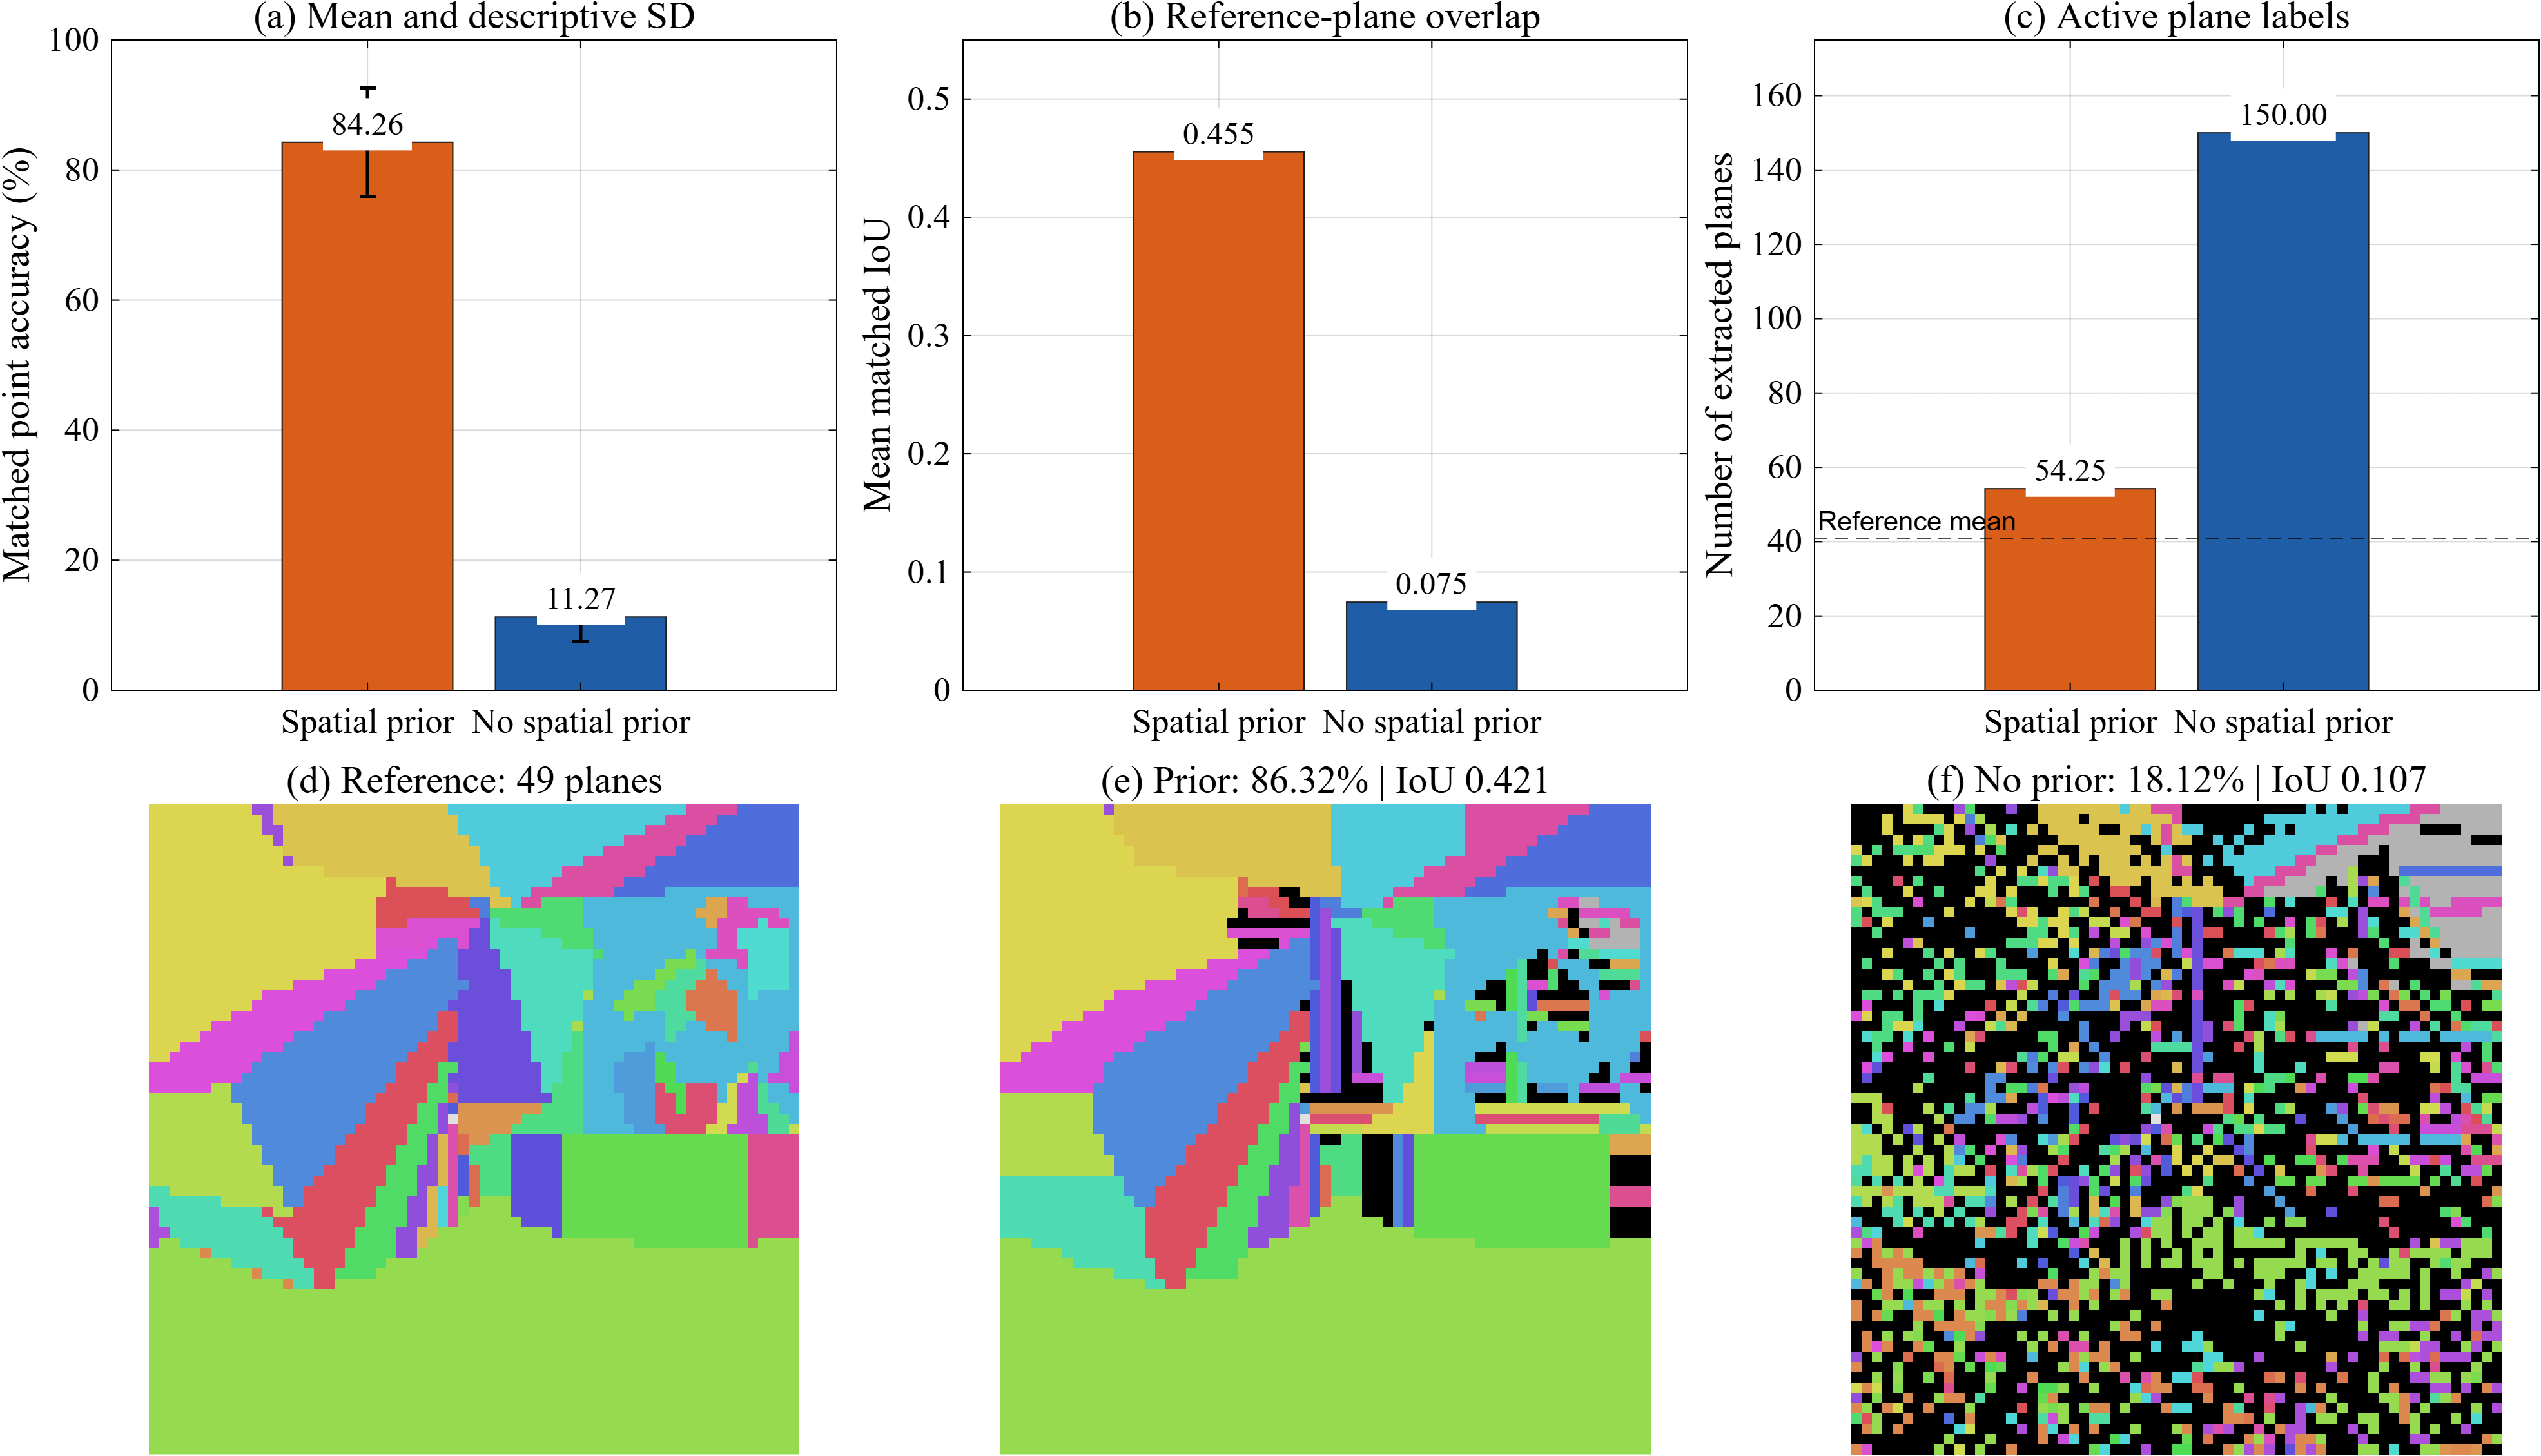
\includegraphics[width=\textwidth]{figures/results_spatial_ablation.png}
\caption{Aggregate ablation results and test pc\_12, var1, seed 7, selected at the lower median regularized accuracy among seed-7 cases. Both conditions use identical saved initial planes. The reference has 49 planes, compared with 74 with the prior and 150 without it. Colors follow Fig.~\ref{fig:results_failure_cases}. The unregularized result shows scattered, incorrect assignments despite SVD refitting.}
\label{fig:results_spatial_ablation}
\end{figure*}

The ablation run records mean times of 36.497 s with the prior and 27.526 s without it. Removing regularization therefore reduces runtime in that run, but the loss of segmentation quality is substantial. Although segmentation scores match the three-way run, its timings differ across sessions; the logs do not establish why. This study makes within-run timing comparisons and does not pool those runtimes.

\subsection{Interpretation and limitations}\label{interpretation-and-limitations}

Under the fixed protocol, refinement usually improves RANSAC, sampled PEARL gives better segmentation at greater cost, and spatial regularization benefits the selected configuration. The initialization experiment changes both models and labels, so it cannot isolate either factor. The \(\eta\) = 0 condition was not separately retuned; tuning it and matching label-visit orders would test the ablation's generality. Correlated records from synthetic scans do not establish significance from 360 independent scenes or real-world robustness. The failures show why point accuracy, overlap, model count, and energy must be interpreted together.

\section{Conclusion}\label{conclusion}

This study has compared sequential RANSAC, sampled-proposal PEARL, and RANSAC-initialized PEARL for multi-plane segmentation on SynPEB. The experiments examine how consensus-based initialization and joint energy minimization affect segmentation quality and computational cost. Their results show that initialization determines both the structures available for refinement and the amount of assignment optimization required.

Among the tested pipelines, the hybrid with confirmed hyperparameters and spatial regularization provides the preferred compromise when computation time and segmentation accuracy are considered together. It achieves 77.98\% mean matched point accuracy in 2.512 s, improving on RANSAC's 69.89\% by 8.08 percentage points. Sampled PEARL achieves the highest accuracy, 84.26\%, but requires 19.620 s on average. The hybrid is therefore approximately 7.81 times faster than sampled PEARL while retaining useful point-level accuracy. Standalone RANSAC remains the fastest option at 0.376 s. These measurements support choosing the hybrid when the additional accuracy of the larger sampled bank does not justify its computational cost.

The runtime decomposition helps explain this tradeoff. The hybrid transfers RANSAC's planes and assignments directly to PEARL and refines a bank containing 19.12 planes on average, compared with 150 initial candidates for sampled PEARL. Its advantage arises mainly during refinement, where fewer labels reduce the expansion workload. Joint reassignment and SVD refitting improve RANSAC point accuracy in 357 of 360 test records. The sampled-proposal ablation further shows the importance of spatial coherence under the selected settings: removing the spatial term reduces mean accuracy from 84.26\% to 11.27\%. Hyperparameters were selected using the training split and fixed before testing; plane parameters and memberships were estimated anew for each scan.

The preferred operating point still has limitations. Hybrid mean matched IoU is 0.2836, below sampled PEARL's 0.4554, indicating incomplete recovery of individual planes despite its reasonable point accuracy. Refinement cannot create additional plane labels, and lower energy does not always improve reference-label accuracy. The findings apply to the synthetic benchmark, sampling policy, and shared parameter selection used here; the unregularized condition was not separately retuned. Further comparisons could examine adaptive additions to the RANSAC model bank, independently tuned ablations, and real scans with explicit plane annotations. Within the present experiment, RANSAC initialization followed by spatially regularized PEARL offers a practical balance between the speed of greedy extraction and the accuracy of joint optimization.

\bibliographystyle{IEEEtran}
\bibliography{references}
\end{document}
